

\begin{abstract}
%!TEX root = /Users/rafaeldurelli/Dropbox/Artigos Elaborados/KDM propagation_2015/sbes_2015_kdm_propagation/sbes2015_kdm_propagation.tex
%
%Architecture-Driven Modernization (ADM) is a model-driven alternative to conventional reengineering processes that relies on the Knowledge-Discovery Metamodel (KDM) as the base for the whole process. Unlike conventional metamodels, KDM is capable of putting together different system abstractions (Code, Architecture, Business Rules, Data, Events) in an unique site and also retaining the dependencies among them. As it is known, central to modernization processes are the refactoring activities. However, most of existing model-based refactorings do not cope with propagation of the refactoring changes across other dependent abstraction levels, keeping all models synchronised. In this paper we present Propagation-Aware Refactorings (PARef), an approach for updating dependent models when specific elements are refactored. Our refactorings involve three main steps; the identification of all dependent elements, the refactoring of them and the propagation of changes in order to keep all the dependent models synchronised. We have conducted an evaluation that shows our refactorings reached good accuracy and completeness levels.
Architecture-Driven Modernization (ADM) is a model-driven alternative to conventional reengineering processes that relies on the Knowledge-Discovery Metamodel (KDM) as the base for the whole process. Unlike conventional metamodels, KDM is capable of putting together different system views (Code, Architecture, Business Rules, Data, Events) in an unique site and also retaining the dependencies among them. During the system life cycle, artifacts tend to change, usually these changes entail refactorings. However, as a system can be represented by several different models, a common accident that arises during refactorings is to desynchronize (inconsistent views) the models. One solution is to apply Static Change Propagation (SCP) techniques. Most of existing SCP techniques deal with propagating changes in different and external models, usually from another vendor preventing or making difficult their application in other models, like KDM. Currently there is a lack of research concentrated on investigating SCP in KDM. In this paper we present a tool-supported KDM-specific approach for updating dependent models/views when specific elements are refactored. Our approach involve three main steps: \textit{i}) identifying diff between the refactored KDM instance and the original KDM instance (the instance before one applies a KDM refactoring), \textit{ii}) the identification of all affected KDM model elements (dependent on the refactored ones), and \textit{iii}) the application of changes (propagation) in order to keep all the models/views synchronized. We have conducted two evaluation that shows our approach reached good accuracy and completeness levels.
\end{abstract}
% IEEEtran.cls defaults to using nonbold math in the Abstract.
% This preserves the distinction between vectors and scalars. However,
% if the conference you are submitting to favors bold math in the abstract,
% then you can use LaTeX's standard command \boldmath at the very start
% of the abstract to achieve this. Many IEEE journals/conferences frown on
% math in the abstract anyway.

% no keywords




% For peer review papers, you can put extra information on the cover
% page as needed:
% \ifCLASSOPTIONpeerreview
% \begin{center} \bfseries EDICS Category: 3-BBND \end{center}
% \fi
%
% For peerreview papers, this IEEEtran command inserts a page break and
% creates the second title. It will be ignored for other modes.
\IEEEpeerreviewmaketitle

\section{Introduction}
	%!TEX root = /Users/rafaeldurelli/Dropbox/Artigos Elaborados/KDM propagation_2015/sbes_2015_kdm_propagation/sbes2015_kdm_propagation.tex

%In 2003 the Object Management Group (OMG) created a task force called Architecture Driven Modernization Task Force (ADMTF). It aims to analyze and evolve typical reengineering processes, formalizing them and making them to be supported by models [2]. ADM advocates the conduction of reengineering processes following the principles of Model-Driven Architecture (MDA) [22][2], i.e., all software artifacts considered along with the process are models.                                       	

%According to OMG the most important artifact provided by ADM is the Knowledge Discovery Metamodel (KDM). By means of it, it is possible to represent different system abstraction levels by using its models, such as source code (Source and Code models), Actions (Action model), Architecture (Structure Model) and Business Rules (Conceptual Model). The idea behind KDM is that the community starts to create parsers and tools that work exclusively over KDM instances; thus, every tool that takes KDM as input can be considered platform and language-independent, propitiating interchange among tools. For instance, a refactoring catalogue for KDM can be used for refactoring systems implemented in different languages. 

%Central to modernization processes are the refactorings. Refactorings are .....  However, most of existing model-based refactorings do not cope with propagation of the refactoring changes across other dependent abstraction levels, keeping all models synchronized [ , , , , ]

%	In this paper we present Propagation-Aware Refactorings (PARef), an approach for updating dependent models when specific elements are refactored.

In 2003 the Object Management Group (OMG) created a task force called Architecture Driven Modernization Task Force (ADMTF). The goal was to analyze and evolve typical reengineering processes, formalizing them and making them to be supported by models~\cite{1686216}. The result of this effort was the creation of Architecture-Driven Modernization (ADM), which advocates the conduction of reengineering processes following the principles of Model Driven Architecture (MDA)~\cite{Heckel2008, Andrade:2005, Reus:2006}, i.e., all software artifacts considered along with the process are models. Therefore, a typical ADM-based modernization process starts with a reverse engineering phase to recuperate a model representation of the system; proceeds by applying refactorings over the recuperated model and finalize by a forward engineering phase where the modernized system is generated.

Knowledge Discovery Metamodel (KDM) is the most important metamodel provided by ADM. Its main characteristics are: i) it is an ISO-IEC standard since 2009 (ISO/IEC 19506); ii) it is platform/language independent, and ii) it is able to represent different views of the same system and retain the dependencies among them by using specific metaclasses. This third point is possible thanks to several internal KDM metamodels/packages that are focused on specific views or abstraction levels, such as  source-code (Code metamodel), behaviors (Action metamodel), architecture (Structure metamodel), business rules (Conceptual metamodel), database (Data metamodel), events (Event metamodel), Graphical User Interface (GUI) (UI metamodel) and deployment (platform metamodel).  

It is well known that refactoring activities are central to modernization processes. Refactorings are defined as the process of modifying the internal structure of software without changing its external observable behavior~\cite{refactImpro}. Behavior preservation in refactoring activities has received a lot of attention for years, both in source code and in models~\cite{4440135, Mens:2006:TMT:1706639.1706924, Mens:2006_NEW, Mens:2007}. One of the known problems when refactoring models is change propagation, i.e., the modifications that need to be done in model elements that are dependent on the refactored model element. Although the behavior preservation is harder to check and characterize when dealing with models, there are works that present proposals of keeping the behavior models updated when static models are refactored~\cite{ICSOFT2014_Winetzhammer}. Most of the works propose solutions to propagate changes across different metamodels not in the same metamodel. 

%However, although some research has been conducted on the theme of change propagation in models~\cite{4440135, Mens:2006:TMT:1706639.1706924, Mens:2006_NEW, Mens:2007, ICSOFT2014_Winetzhammer}, none of them have devoted attention on a metamodel like KDM, which groups several metamodels under a unique place and already provide metaclasses for retaining the dependences among these models. In most cases, the related works concentrate on propagating changes in a metamodel different from where had occurred the modification. Besides, the concentration of some of them are in behavior preservation, an aspect that is out of the scope of this work.

However, although some research has been conducted on the theme of change propagation in models~\cite{4440135, Mens:2006:TMT:1706639.1706924, Mens:2006_NEW, Mens:2007, ICSOFT2014_Winetzhammer}, none of them has devoted attention on a metamodel like KDM, which groups several metamodels under a unique place and already provide metaclasses for retaining the dependences among these models. In most cases, the related works concentrate on propagating changes in a different metamodel from where had occured the modification. Besides, the concentration of some of them are in behavior preservation, an aspect that is out of the scope of this work. Furthermore, up to this moment, few research has been done on KDM refactorings~\cite{IRIDurelliCatalogo, 7051941}, limiting the dissemination and adoption of ADM. We believe that our change propagation approach will foster the creation and research on KDM refactorings. 

%In this paper we present an approach for propagating changes when refactoring KDM model instances. The main goal is to guarantee the global system representation keep synchronized along with the refactoring activities; which are much common during modernization processes. Our approach runs in three steps: i) a search algorithm identifies all the KDM metaclasses dependent on the refactored elements and ii) an ATL Transformation Language (ATL) that performs the model transformation/refactoring, and iii) another ATL created to propagate all the changes throughout all KDM's view. This last step was implemented in a generic way - as a decoupled module, which can be coupled to existing refactorings. In this way, existing users can write KDM refactorings in ATL without worrying about the change propagation. The only task is to provide for our component the input it needs to conduct the propagation.

In this paper we present an approach for propagating changes when refactoring KDM model instances. The main goal is to guarantee the global system representation keep synchronized along with the refactoring activities; which are much common during modernization processes. Our approach runs in three steps: i) a mining algorithm identifies all KDM metaclasses that need to be updated when refactoring a specific KDM metaclass, ii) an ATL Transformation Language (ATL) that performs the intended refactoring, and iii) another ATL that performs one or more model transformations that characterize change propagation. We have implemented the approach in a generic way as a decoupled module, which can be coupled to existing refactorings. In this way, existing users can write KDM refactorings in ATL without worrying about the change propagation. The only task is to provide for our component the input it needs to conduct the propagation.

The main contributions are: i) a mining algorithm to identify all KDM metaclasses that need to be updated when a specific refactoring is performed, ii) a set of refactoring devised to KDM domain, iii) a propagation technique approach, and (iv) a support and preliminary infrastructure for allowing the creation of refactorings for kdm.

This paper is structured as follows: In Section~\ref{sec:background} the notion related to ADM and KDM, their details and a system's description that was instantiated in KDM are showed.
%
%
%Section~\ref{sec:background} presents all needed background on ADM and KDM. 
In Section~\ref{sec:motivation_and_running_example} a motivation is presented. Section~\ref{sec:the_approach} shown the proposed approach. In Section~\ref{sec:evaluation}, an empirical evaluation is presented. In Section~\ref{sec:related_work} there are related works and in Section~\ref{sec:conclusion} there are the conclusions.



	%This paper is structured as follows: in Section II, Crosscutting Frameworks are explained; in Section III, the Proposed Model and the Reuse Process are shown; in Section IV, a tool to support the process is used to reuse a persistence framework as an Example; in Section V, an empirical evaluation is presented; in Section VI, there are related works and in Section VII, there are the conclusions.

%!TEX root = /Users/rafaeldurelli/Dropbox/Artigos Elaborados/KDM propagation_2015/sbes_2015_kdm_propagation/sbes2015_kdm_propagation.tex

\section{ADM and KDM} % (fold)
\label{sec:background}
 
\begin{figure*}[t]
	\centering
	% Requires \usepackage{graphicx}
	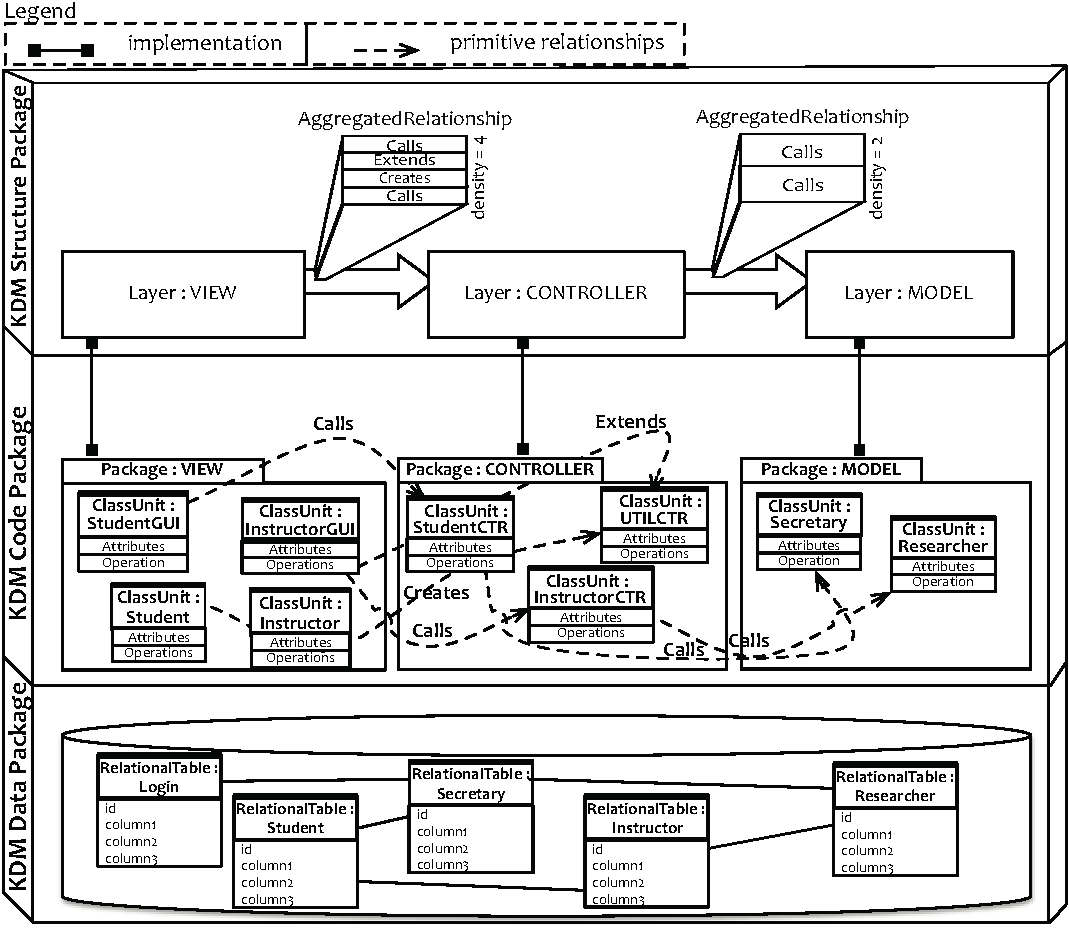
\includegraphics[scale=0.8]{figuras/NovoSystem3}
	\caption{System example.}
	\label{fig:system}
\end{figure*}

ADM is the process of understanding  and evolving existing software systems taking model-driven principles into account~\cite{1686216}. A typical ADM process involves three main phases: Reverse Engineering, Refactorings/Optimizations and Forward Engineering. In reverse engineering, a legacy system is abstracted in a KDM instance. Next, some refactorings and optimizations can be applied over the KDM instance and, in the last phase, the modernized source code is generated. 

KDM is the most important meta-model of ADM (ISO/IEC 19506), providing a comprehensive view of as-is application and data architectures, into a unique meta-model. This is different from conventional model-driven development techniques we have found on literature~\cite{7051941}, since many of them employs several meta-models, from different vendors, along the process~\cite{Perez-Castillo:2011:KDM}. KDM can be seen as a family of meta-models, as it contains twelve packages; each one representing a meta-model that concentrates on a different view of the system. Thus, by using its  meta-models, it is possible to have a number of views of a system. For example, it is possible to have a low level system representation, describing source-code details and several others views of the system, such as an architectural view, a data view, a business rule view, a behavioral view, etc. Moreover, as KDM groups a set of meta-models, all of them share the same terminology, i.e., all of the meta-models know the main meta-model elements, such as ClassUnit, KDMEntity and MethodUnit, etc.

Considering the scope of this paper, some important KDM packages are Code, Structure, Data and Conceptual. Code package provides a lot of meta-classes for representing source code details, such as MethodUnit (methods), ClassUnit (classes) and StorableUnit (attributes). Structure package is devoted to represent the architecture of the system, employing architectural concepts commonly find in the literature. So, it offers meta-classes for representing layers (Layer meta-class), subsystems (Subsystem meta-class), components (Component meta-class) and architecture views (ArchitectureView meta-class). It also offers a special kind of relationship called Aggregated (AggregatedRelationhip meta-class), whose goal is to relate architectural elements with each other. An important characteristic of this relationship is that it acts as a container of primitive relationships, i.e., it is possible to group several primitive relationships within it. 

Data package aims at representing the database structure of the system, providing meta-classes for representing tables and their attributes (Columns, primary key, etc). Conceptual package offers meta-classes for representing conceptual elements of a system, such as business rules (RuleUnit meta-class), scenarios (Scenario meta-class), etc. 

The main goal is to allow a complete representation of systems, ranging from low to high-level views. All of the aforementioned meta-models, although being in different abstraction levels, can be interrelated to each other. For example, consider the existence of a Java package P1 (Package meta-class) that contains a class C1 (ClassUnit meta-class). This package can be the source-code realization of a Layer L1 (Layer meta-class) and, at the same time, the realization of a Scenario S1. The class C1 can also be the realization of a business rule B1 (RuleUnit meta-class) that is inside the scenario S1. 

\section{A Running Example}\label{sec:running_example}

Figure~\ref{fig:system} presents an example that is used throughout this paper. It is shown schematically how KDM can be used for representing three views/abstractions of part of an Academic Management System: Code View, Architecture View and Data View. The entire figure represents a KDM model, i.e., an instance of KDM composed by three other internal instances - each of the three big rectangles represents an instance of an internal meta-model. So, there is an instance of the Code meta-model (middle), another instance of the Structure meta-model (upper part) and another one of the Data meta-model (lower part). 

Besides, each of the smaller internal elements (classes, packages, layers, relationships, etc) contains also instances of KDM meta-classes. Notice we are using the pattern \textbf{instance name: Meta-class name} in the name of every element so that the name of the meta-class can be seen. As this is an MVC-based system, Code View contains three instances of the Package meta-class: VIEW, CONTROLLER and MODEL. Each of them involving some ClassUnit instances. The classes are related to each other by means of static (associations, inheritance, interface realizations and imports) or dynamic (calls, object creation, parameter passing, etc) relationships. Each of these relationships is also an instance of specific meta-classes. 

The Architecture View represents the system architecture. In this example each smaller rectangle represents an instance of a meta-class called Layer. The system is organized in three layers:  VIEW, CONTROLLER, and MODEL. Between Layes and Packages there are a set of relationship called \texttt{Implementation}, which are represented in Figure~\ref{fig:system} by the symbol \foobarMeu. The intention of this type of relationship is to denote that a specific higher-level abstraction is realized by one or more lower level code elements. In this example, the Layer View is realized in source-code level by the package VIEW; the Model layer is realized by the package Model and the layer Controller by the Controller package. The \texttt{Implementation} relationship is very important in this work, as it is the main link between meta-models in different abstraction levels. Observe in the figure that the unique route between the views are by means of these relationships.

KDM also possesses an important relationship type called AggregatedRelationship whose aim is to represent dependencies between architectural elements of the Structure Package. Using this relationship it is possible to put together several primitive relationships in a unique ``channel''. For example, there are thicker relationships between the layers representing the AggregatedRelationship. It is also possible to see that these relationships aggregate some primitive relationships. For example, the AggregatedRelationship between the layer View and the layer Controller group the following relationships: two Calls, one Creates and one Extends. The number aside the AggregatedRelationship is called density, that represents the amount of primitive relationships exists inside it.

Finally, the Data Package depicts the system s database and its tables. Herein, it is possible to notice that the depicted system owns a set of Plain Old Java Objects (POJOS), they are: Student, Instructor, Secretary, and Researcher. All of these POJOS are also Object Relational Mapping (ORM), i.e., they are mapped to the Data package using the meta-class RelationalTable and its columns are mapped using the meta-classes UniqueKey and ColumnSet.

An evident problem in this example is the presence of the classes \texttt{Student} and \texttt{Instructor} in the VIEW package. A possible solution to this problem is to apply the \textit{Move Class} KDM refactoring as presented in Figure~\ref{fig:ATLRefactoring}.

\begin{figure}[h]
	\centering
	% Requires \usepackage{graphicx}
	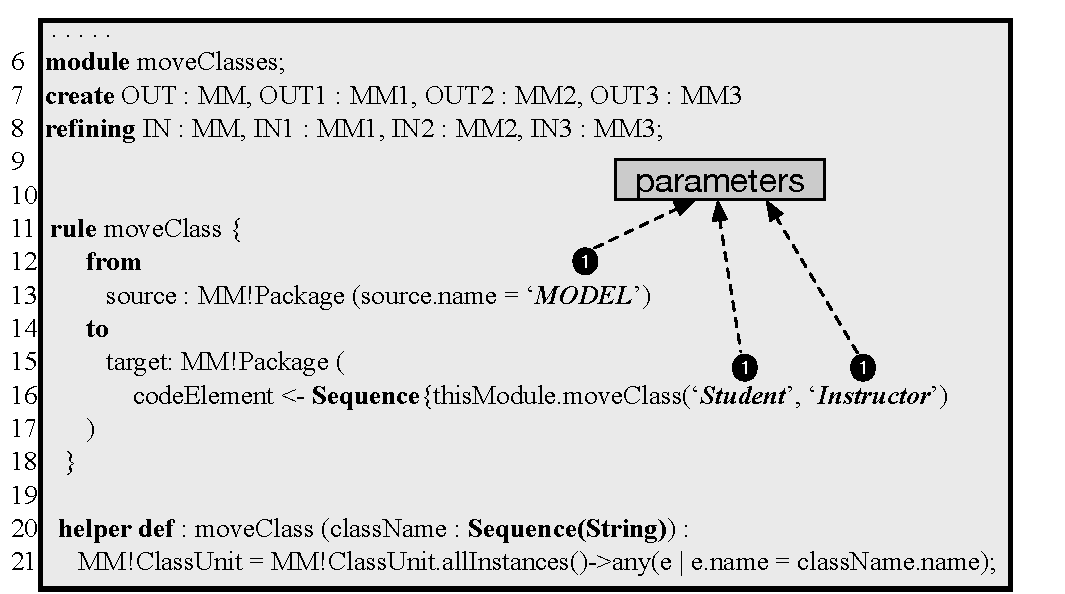
\includegraphics[scale=0.516]{figuras/moveClassRefactoringFormatted}
	\caption{Chunk of code in ATL to perform the refactoring \textit{Move Class}.}
	\label{fig:ATLRefactoring}
\end{figure}

Lines 14 though 19 the \textit{Move Class} is actually defined. Lines 21 and 22 there is a helper, in ATL helpers are like methods in programing languages. This helper is used to verify if the ClassUnit is the correct class to be moved. 
Almost all refactorings need some input parameters that should be properly informed by the user. For instance, in the code depicted in Figure~\ref{fig:ATLRefactoring}, lines 13, 16, and 17 the software modernizer informed three parameters (see \ding{182}), i.e, he(she) specified the source Package and two ClassUnits that he(she) would like to move.
Afterward, this ATL is ready to be applied into a KDM instance.

Observing the refactoring defined in Figure~\ref{fig:ATLRefactoring} it is fairly evident that both classes \texttt{Student} and \texttt{Instructor} should be moved to the MODEL package.
%
%During a refactoring activity, these classes should be moved to the Model package. 
However, moving these classes will turn the KDM instance inconsistent, because the ``density'' value will turn wrong, i.e., AggregationRelationShip between
the layer VIEW and the layer CONTROLLER would
change from 4 to 2 - once the primitives relationships Creates
and Extends would no longer exist from the package VIEW
to the package CONTROLLER. In the same way, the result of \textit{Move Class} refactoring should also update the density between the layer
MODEL and CONTROLLER, instead of 2 it should be 4, as
Creates and Extends were also moved along with its
classes, \texttt{Student} and \texttt{Instructor}.

These propagation seen to be easy to apply, however, in a complex system comprising all kdm's packages/levels propagate all changes after a refactoring is a difficult and error prone task. Even identifying the affected parts of the KDM's packages/levels is not an easy and straightforward process. A typical refactoring written in ATL is shown in Figure~\ref{fig:ATLRefactoring}.

%--------------valters background---------------------------------------




%----------------------------------------------------------------------

%In this section we provide a brief background to Architecture-Driven Modernization (ADM) and Knowledge Discovery Metamodel (KDM). 

%Further, we describe in detail why change propagation in KDM is a complex process.

%\subsection{ADM and KDM}

%The growing interest in using MDA to manage software evolution~\cite{Heckel2008, Andrade:2005, Reus:2006} 
%
%
%is mainly focused on the reengineering or modernization of legacy systems. Several software migration projects have been carried out with model-driven approaches~\cite{Heckel2008, Andrade:2005, Reus:2006}. %In addition, the 
%This interest 
%motived OMG to define the Architecture-Driven Modernization (ADM) initiative~\cite{1686216} which advocates carrying out the reengineering process considering models. 
%
%ADM is the concept of modernizing existing systems with a focus on all aspects of the current systems architecture and the ability to transform current architectures to target architectures by using all principles of MDD~\cite[p.~60]{Ulrich:2010:IST:1841736}. 
%
%
%Figure~\ref{fig:ADM_shorseshoe} depicts the horseshoe model (i.e., horseshoe is basically a left-hand side, a right-hand side and a bridge between the sides) adapted to ADM. %Please note that it contains all the traditional phases and some MDD's keywords, such as PSM and  PIM. The traditional phases adapted to ADM are:
%\begin{figure}[!ht]
%\centering
  % Requires \usepackage{graphicx}
% 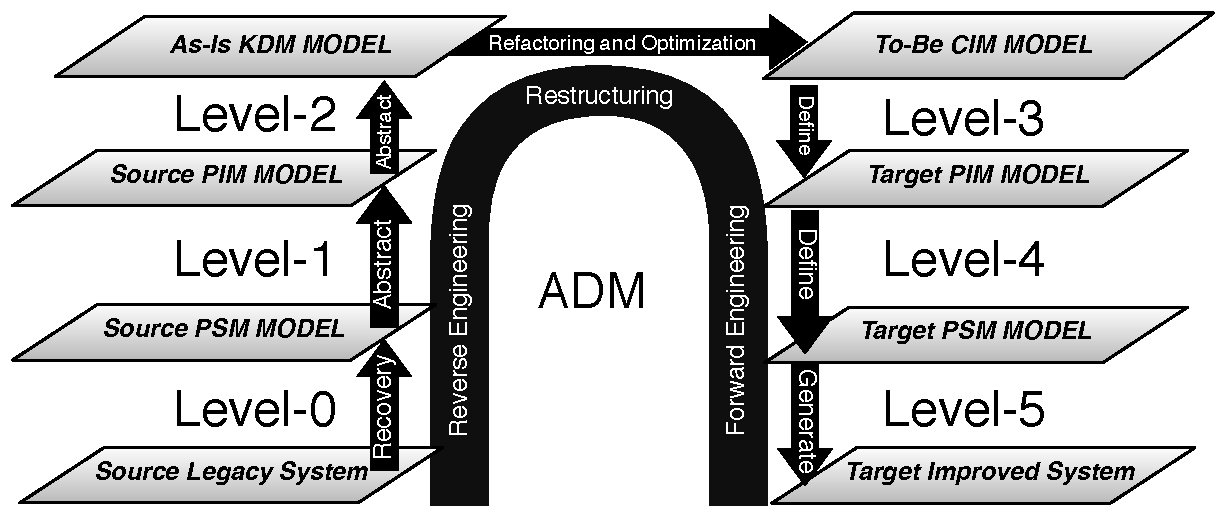
\includegraphics[scale=0.42]{figuras/processoDaFerramenta}
%\caption{Horseshoe Modernization Model~\cite{OMG_ADM}.}
%\label{fig:ADM_shorseshoe}
%\end{figure}
%This horseshoe model contains three main phases. The first one is the \textbf{Reverse Engineering} that takes a legacy system to be modernized as input.  Further the knowledge is extracted and a Platform-Specific Model (PSM) is generated. Next, this PSM serves as the basis for the generation of a Platform-Independent Language (PIM), which is called KDM. The second phase is the \textbf{Restructuring}, in which a set set of reengineering/refactoring can be applied into a KDM's instance by means of model transformations. The third phase is the \textbf{Forward Engineering} where a forward engineering is carried out and the source code of the modernized target system is generated.

%Figure~\ref{horseshoe} depicts the ADM modernization domain model where the left side of the horseshoe is the current state of a busines/it architecture ``as is'' and the right side is what we want to get after the modernization ``to-be''. %One common path followed by IT is to focus on the technical architecture. Generally, the cost of this approach is lower and project duration shorter because the data and application architectures remain largely intact but there is almost no impact or value to the business. 

%On the other hand, a modernization which seeks to provide value to the business, would need to change the application and data architecture, which in turn would rely on an analysis of requirements stemming from shifts to the business architecture. These types of projects are of a longer duration, require more investment, and deliver significantly more value to the business.




%To perform a systematic modernization as depicted in Figure~\ref{fig:ADM_shorseshoe}, ADM introduces several modernization standards, among them there is the Knowledge Discovery Metamodel (KDM).
%However, herein we focus on KDM because it is the key cornerstone of ADM and the main ideas of our research.  KDM is an OMG specification adopted as ISO/IEC 19506 by the International Standards Organization for representing information related to existing software systems. The goal of the KDM standard is to define a metamodel to represent all the different legacy software artifacts involved in a legacy information system (e.g. Code, Architecture, Business Rules, Data, Events, etc.). %The metamodel of the KDM standard provides a comprehensive high-level view of the behavior, structure and data of legacy information systems by means of a set of facts. 

%KDM contains twelve packages and it is structured in a hierarchy of four layers: (\textit{i}) Infrastructure Layer, (\textit{ii}) Program Elements Layer, (\textit{iii}) Runtime Resource Layer, and (\textit{iv}) Abstractions Layer. These layers can be instantiated automatically, semi-automatically or manually through the application of various techniques of extraction of knowledge, analysis and transformations~\cite{1686216}. Figure~\ref{fig:kdmLayers} depicts the architecture of KDM and its layers. %By observing this figure it is fairly evident that each layer is based on the previous layer. 
%They are organized into packages that define a set of metamodel, whose purpose is to represent a specific and independent interest of knowledge related to legacy systems, e.g. source code, user interfaces, databases, business rules, etc.

%\begin{figure}[!ht]
%\centering
  % Requires \usepackage{graphicx}
 %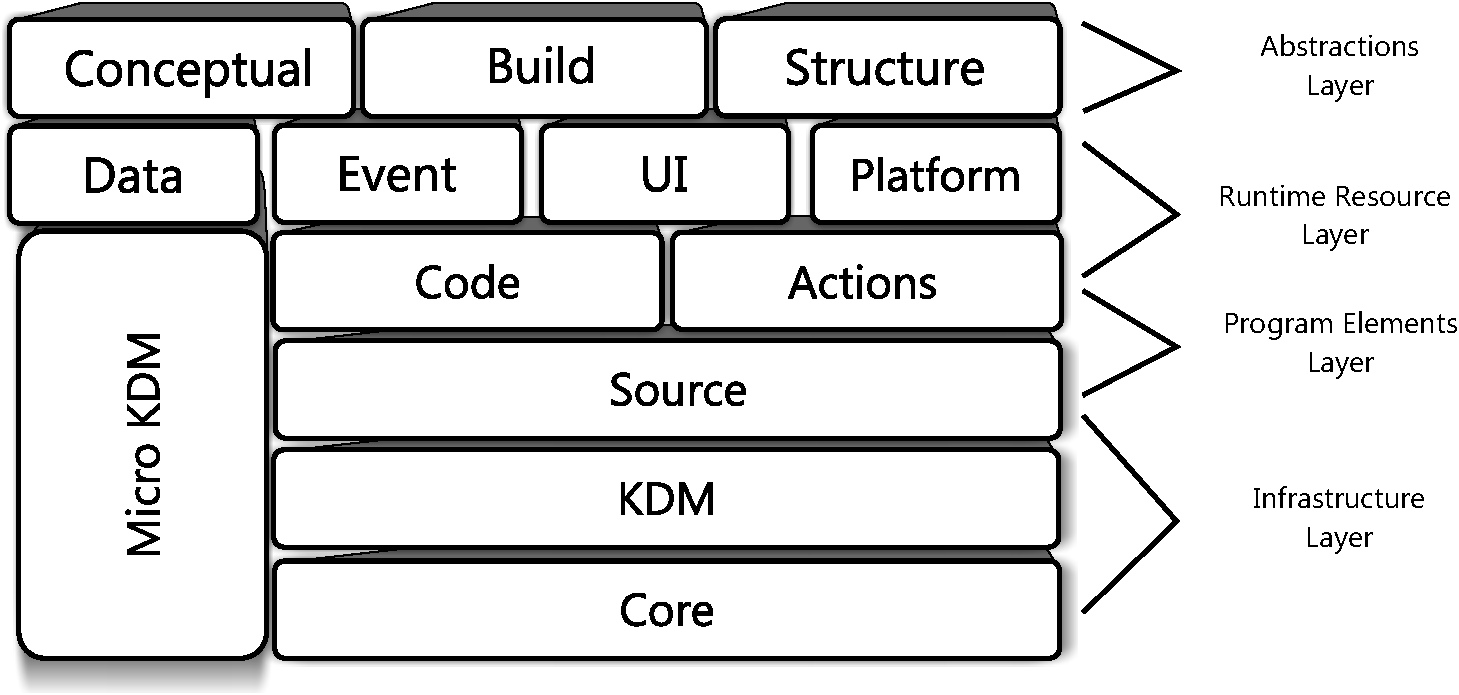
\includegraphics[width=3.3in]{figuras/camadas_kdm}
%\caption{KDM Architecture.}
%\label{fig:kdmLayers}
%\end{figure}

%Although KDM is a metamodel to represent a whole system, its main purpose is not the representation of models related strictly to the source code nature such as Unified Modeling Language (UML). While UML can be used to generate new code in a top-down manner, an ADM-based process using KDM starts from the different legacy software artifacts and builds higher-abstraction level models in a bottom-up manner through reverse engineering techniques. %KDM can be seen from different perspectives, as follows: (\textit{i}) KDM can be considered as a metamodel to represent legacy knowledge models, (\textit{ii}) most of the KDM specification is a definition of a language- and platform-independent ontology of legacy information systems and (\textit{iii}) KDM is a common interchange format that makes the interoperability between the reverse engineering tools and modernization tools possible.

%KDM specification owns some KDM domain, each domain defines an architectural viewpoint. In order to define the catalogue of refactoring for the KDM we need to focus just on the Program Element Layer - more specifically  in the Code Package, which represents the code elements of a program (classes, fields and methods) and their associations. %We are interested in the Code Package once our catalogue is based on fine-grained refactorings, i.e., refactorings to be applied into classes, fields and methods. 
%Therefore, it is important to dig a little deeper in the Code Package.
%
%In a given KDM instance, each instance of the code meta-model element represents some programming language construct, determined by the programming language of the existing software system. Each instance of a code meta-model element corresponds to a certain region of the source code in one of the artifacts of the existing software system. In addition, 
%
%The Code Package consists of $24$ classes and contains all the abstract elements for modeling the static structure of the source code. In Table~\ref{tab:mappingCodeToKDM} is depicted some of them. This table identifies KDM metaclasses possessing similar characteristics to the static structure of the source code. Some metaclasses can be direct mapped, such as Class from object-oriented language, which can be easily mapped to the ClassUnit metaclass from KDM.


%\begin{table}[!h]
%\caption{Metaclasses for modeling the static structure of the source-code}
%\label{tab:mappingCodeToKDM}
%\centering
%\begin{tabular}{|>{\centering}p{3cm}|>{\centering}p{3cm}|}
%\hline 
%Source-Code Element & KDM Element\tabularnewline
%\hline 
%\hline 
%Class & ClassUnit\tabularnewline
%\hline 
%Interface & InterfaceUnit\tabularnewline
%\hline 
%Method & MethodUnit\tabularnewline
%\hline 
%Field & StorableUnit\tabularnewline
%\hline 
%Local Variable & Member\tabularnewline
%\hline 
%Parameter & ParameterUnit\tabularnewline
%\hline 
%Association & KDM RelationShip\tabularnewline
%\hline 
%\end{tabular}
%\end{table}

  %\begin{figure}[!ht]
  %\centering
  % Requires \usepackage{graphicx}
    %\includegraphics[scale=0.39]{FIGURAS_DA_REFATORACAO/ProgramLaye0r}
  %\caption{Chunk of the Code Package (OMG Group~\cite{OMGADM})}
  %\label{fig:programLayer}
  %\end{figure}

 %As can be seen in Figure~\ref{fig:programLayer} the root metaclass is \textit{ComputationalObject} which has two sub-metaclasses, i.e., \textit{DataElement} and \textit{ControlElement}. The former sub-metaclass, \textit{DataElement}, is a generic modeling element that defines the common properties of several concrete classes that represent the named data items of existing software systems, for example, global and local variables, record files, and formal parameters. \textit{DataElement} has five sub-metaclasses - \textit{StorableUnit}, \textit{IndexUnit}, \textit{ItemUnit}, \textit{ParameterUnit} and \textit{MemberUnit}. \textit{StorableUnit} is a concrete  sub-metaclass of the \textit{StorableElement} meta-class that represents variables of the existing software system. \textit{IndexUnit} class is a concrete subclass of the \textit{DataElement} class that represents an index of an array datatype. Instances of \textit{ItemUnit} class are endpoints of KDM data relations which describes access to complex datatypes. \textit{ParameterUnit} class is a concrete subclass of the \textit{DataElement} class that represents a formal parameter; for example, a formal parameter of a procedure. \textit{MemberUnit} class is a concrete subclass of the \textit{DataElement} class that represents a member of a class type. Finally, the latter, \textit{ControlElement} is a sub-metaclass that contains two sub-metaclasses - \textit{MethodUnit} and \textit{CallableUnit}. \textit{MethodUnit} element represents member functions owned by a \textit{ClassUnit}, including user-defined operators, constructors and destructors. The \textit{CallableUnit} represents a basic stand-alone element that can be called, such as a procedure or a function. %As can be seen below the dashed line in Figure~\ref{fig:programLayer} there are also the following enumerations: ``\textit{ExportKind}'', ``\textit{StorableKind}'', ``\textit{CallableKind}'', ``\textit{MethodKind}'', which are sets os literals used as properties of the metaclasses.


	

%%!TEX root = /Users/rafaeldurelli/Dropbox/Artigos Elaborados/KDM propagation_2015/sbes_2015_kdm_propagation/sbes2015_kdm_propagation.tex
\section{Motivation} % (fold)
\label{sec:motivation_and_running_example}

%In our previous work~\cite{IRIDurelliCatalogo}, we introduced a refactoring catalogue for KDM for managing evolution of a software system. This catalogue served as a starting point to investigate how the changes affect the KDM's levels. 

Considering the system described earlier it is possible to identify two refactoring opportunities. The first one is related to the \texttt{Student} and \texttt{Instructor} classes, which are erroneously in the \texttt{VIEW} package and should be moved to the \texttt{MODEL} package using the  \textit{Move Classes} refactoring. The second one is regarding the attributes of the \texttt{Student} class that represent an address. A possible structural improvement could be turned these attributes into a new class Address - so the \textit{Extract Class} can be applied here. 

%remark some problem or even to add new requirements that will propagate changes at KDM's levels. For instance, a problem that can be noticed is that both classes \texttt{Student} and \texttt{Instructor} ( see figure~\ref{fig:system} \ding{182}) should be contained in \texttt{Model} package not in \texttt{GUI} package, respectively. One way to fix this would be to apply the refactoring \textit{Move Class}. Then both classes should be moved to the correct package.
%
%
%
%
%Regarding to a new requirement let's pretend someone has identified that the class 	\texttt{Student} is doing work that should be done by two classes, e.g., it contains attributes that hold informations upon student's addresses. In order to fulfill this new requirement one should apply the refactoring \textit{Extract Class}. Then a new class named Address would be created (which is a POJO and also an ORM) and all student's attributes related to address would be moved to this new class.

%The action of this refactoring should propagate throughout other KDM's levels, such as the data level\footnote{The KDM's level that contains information on data base schema, table, column, primary key, etc}. 
However, these changes would rise a synchronization problem among all KDM's levels/packages. For instance, in both described refactoring it is necessary a skilled domain expert into KDM to identify all the metaclasses in the system which involve/reference the classes aforementioned and correct them respectively in all KDM packages.%, i.e., propagate all refactoring's impact throughout all KDM's packages/level. 

In the matter of the refactoring \textit{Move Class} (move \texttt{Student} and \texttt{Instructor} from \texttt{VIEW} package to \texttt{MODEL} package) changes should be propagated to the \texttt{Structure Package} and to the \texttt{Conceptual Package} to maintain the model synchronized. Regarding the \texttt{Structure Package}, the \texttt{density}, i.e., aggregation relation ship between the layer \texttt{View} and the layer \texttt{Controller} would change from 4 to 2 - once the primitives relationships \texttt{Create} and \texttt{Extends} would no longer exist from the package \texttt{VIEW} to the package \texttt{CONTROLLER}. On the other hand, the resulting of this refactoring would update the density between the layer \texttt{Model} and \texttt{Controller}, instead of 2 it should be 4, as \texttt{Creates} and \texttt{Extends} were also moved along with its classes, \texttt{Student} and \texttt{Instructor}. Concerning to the \texttt{Conceptual Package}, the  RuleUnit\_1.1 that is associated with \texttt{Instructor} should also be moved to corresponding scenario, i.e, the scenario that is associated with the package that contains now the class \texttt{Instructor} - ScenarioUnit\_3. 

About the refactoring \textit{Extract Class}, the extracted class \texttt{Address} would be a POJO (it would be contained in \texttt{Model package} and it would also be an ORM - therefore, the action of this refactoring should be propagated throughout  the \texttt{Data package}, i.e., the instance of \texttt{Address} should be associated with a metaclass \texttt{RelationalTable}, and its attributes should be associated with  of \texttt{ColumnSet}.

%, i.e., the relationship among the layers should be propagated automatically. Similarly, considering the refactoring \textit{Extract Class}, where a new POJO and ORM class is created, the data's level also should be propagated.

%These propagation seen to be easy to apply, however, in a complex system comprising all kdm's packages/levels, propagate all changes after a refactoring is a difficult and error-prone task. Even identifying the affected parts of the KDM's packages/levels is not an easy and straightforward process. 

%-------------------------
In the context of model-driven  refactoring, if any change occurs at any KDM's subtree the change should be propagated to other elements.
%
%These levels indicate problems related to KDM propagation of changes. 
%
For instance, when the elements of \texttt{CodeModel} suffer any kind of changes, its instances, i.e., \texttt{ClassUnits}, \texttt{MethodUnits}, \texttt{StorableUnits}, etc, and related elements must be adapted accordingly so that their validity and correctness is preserved respectively. In addition, if we want to preserve others parts of KDM, like the system's structure and the business rules the  \texttt{StructureModel} and \texttt{ConceptualModel} also need to adapt, respectively. %What is more, as we have mentioned, in practice there are usually at least one instance of each KDM's model applied in a single system, e.g., the system architecture conforms to Structure Model, the source-code conforms to Code Model, etc. 
In general, a change at one KDM's package/level should trigger a cascade of changes at other models. We call such sequences of adaptations change propagation.

%As we can see in Figure~\ref{fig:allKDMLayers}, there are not only horizontally relations between the models, but the elements of the system can also be vertical related across the vertical partitions. A few examples are denoted by the red/blue dashed arrows. For instance, there is a relation between a \texttt{CodeModel} (its respective metaclasses) with the \texttt{StructureModel} - which means that a change in one of the ends of the relation can influences the other.

Considering these KDM's models as individual artifacts lead up to refactoring of each affected model separately, causing synchronization problem among them. However, this is an error-prone solution since we need to apply a refactoring at any KDM's models and then propagate all change in order to keep a KDM instance synchronized. %a domain expert who is able to identify all the affected models and propagate the changes. 
%In this context, we present an approach to detect and propagate all the changes throughout all KDM's levels after one to apply a refactoring 

%-------------------------

%In order to fulfill this limitation and create an automatized process named Propagation-Aware Refactorings (PARef) that contains three main steps. The first step is the identification of all dependent elements related to a specific refactoring. In the second step the refactoring of all identified elements are performed using a model-to-model transformation language - the third step is the propagation of changes in order to keep all the dependent models synchronized. %In the following sections we show in detail that change propagation in KDM is a complex process that can be solved semi-automatically and, hence, efficiently and precisely if we provide a rigorous theoretical background. In the following sections our approach is presented.
 
	

%!TEX root = /Users/rafaeldurelli/Dropbox/Artigos Elaborados/KDM propagation_2015/sbes_2015_kdm_propagation/sbes2015_kdm_propagation.tex

\section{Propagation-Aware Refactorings} % (fold)
\label{sec:the_approach}

In order to fulfill the limitation pointed out, we introduce an approach that aims to propagate all the changes throughout the KDM's levels. This approach ensures that when a change/refactoring is performed in any KDM's level, it is correctly propagated to the affected KDM's levels and vice versa. So it make certain that the consistency between the KDM's levels when they are refactored. 
The described problem presented in Section~\ref{sec:motivation_and_running_example} can, in our view, be split into three steps, which are depicted by its corresponding letters and tittle in Figure~\ref{fig:approach}. 

%According to the literature, there are two possibilities to perform propagation in models (colocar ref). One possibility is to mark the modifications on the source KDM's model without actually commiting them until the end of the transformation, so that expression evaluation can occur on the original source KDM's model by ignoring the modifications. Another possibility is to first compute the set of basic operations to perform, storing this set in an external artifact representation and then apply all the changes at once. Our approach follows the second possibility and it is divided in three steps, which are depicted by its corresponding letters and tittle in Figure~\ref{fig:approach}.


\begin{figure}[h]
	\centering
	% Requires \usepackage{graphicx}
	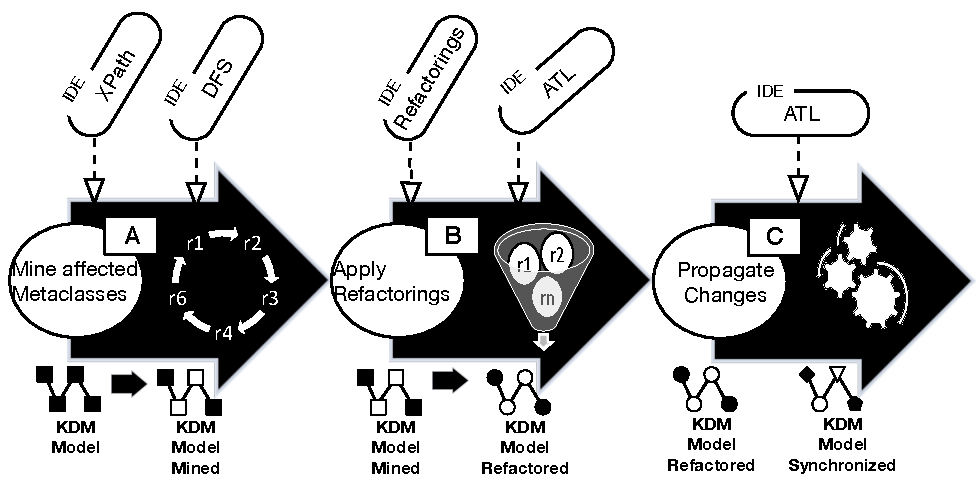
\includegraphics[scale=0.56]{figuras/allStepApproachKDMPropagation}
	\caption{Propagation-Aware Refactorings steps.}
	\label{fig:approach}
\end{figure}

In the step [A], \textit{Mine Affected Metaclasses}, we developed a mechanism which shows all metaclasses that need to be updated after applying any changes/refactoring. These metaclasses are those that have some dependence on the metaclass to be modified by the refactoring. This step is totally based on a set of queries that works on a KDM instance. In fact, this step uses depth-first search algorithm to identify all affected metaclasses along with a set of queries.

In step [B], \textit{Apply Refactoring}, here the software modernizer has to choose an appropriate refactoring to be applied into the KDM. In this step, new metaclasses can be created, updated, and removed. Also it is necessary to gather all the needed parameters for applying the refactoring. %that the software modernizer inputs all the needs parameters for applying the refactoring is gathered.  %The most frequent modification to the KDM instances in this scenario will be, intuitively, creating new metaclasses. However, updating existing metaclasses with their relationship will be frequent as well. In simpler cases, updating means changing properties of existing metaclasses. In more complex cases, updating means removing metaclasses and replacing them with new and refactored ones.
This step uses M2M transformation language to perform the refactorings.

In step [C], \textit{Propagate Changes}, involves updating the elements identified in the step [A].  As in step [B], in this step we also have used M2M to update all KDM's instances. 
More details on each step are provided in the next sections.

\subsection{Mine Affected Metaclasses} % (fold)
\label{sub:mine_affected_metaclasses}

The step [A] starts with a depth-first search algorithm that aims to show all metaclasses and its relationships that use somehow the metaclass(es) that will be refactored in step [B]. As input all the metaclasses that will be used to apply an specific refactoring is needed. The algorithm uses a set of queries. These queries are performed on the KDM's instance to mine all the affected/linked metaclasses. All the queries were created using XPath. We have decided to use XPath because it is a well-know and well-documented language. 

Let us consider the running example depicted in Figure~\ref{fig:system}. In this example, the engineer aims to apply the refactoring \textit{Move Class} - both classes \texttt{Student} and \texttt{Instructor} should not longer be contained in the package \texttt{View}. These classes should be allocated into the package \texttt{Model}. Considering the refactoring \textit{Move Class}, three elements (\texttt{Student}, \texttt{Instructor}, and their package) need to be investigated throughout the KDM's instance in order to identify propagation scenarios of changes. 

Therefore, firstly a query must be executed to get the root elements in KDM. This query is represented as the first statement in Figure~\ref{fig:queriesXPath}, see line 1 - it is used to return an instance of the metaclass \texttt{Segment}. The returned Segment, as well as all KDM's levels are gathered by the other queries presented in Figure~\ref{fig:queriesXPath} lines 2 to 5. The returned elements of these queries are used as input in our depth-first search algorithm.

\begin{figure}[h]
	\centering
	% Requires \usepackage{graphicx}
	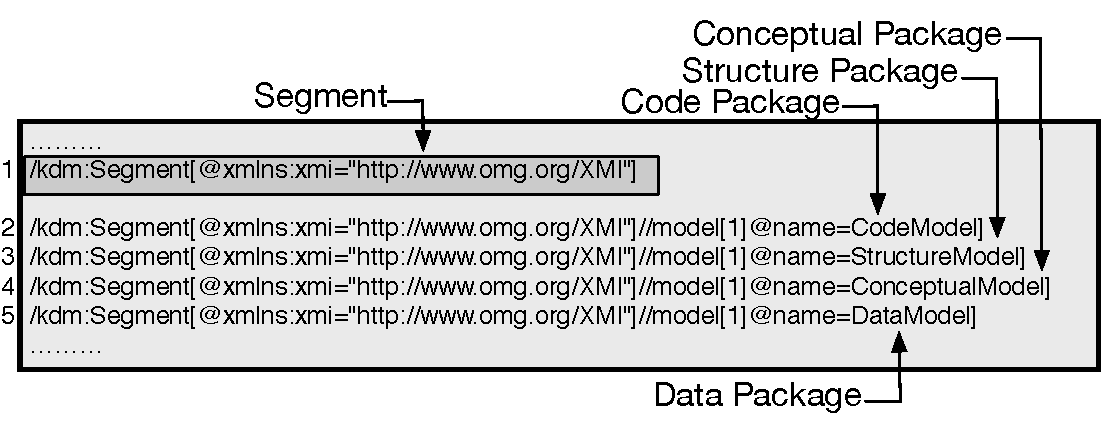
\includegraphics[scale=0.479]{figuras/queiresANDATLSBESNew}
	\caption{Xpath used to return the KDM's root element, Segment.}
	\label{fig:queriesXPath}
\end{figure}


\begin{algorithm}[h]
     \SetAlgoLined
     \KwIn{DFS (G, u, eL) where G is a KDM's instance, u is the initial metaclass, i.e., Segment, and eL is a set of elements to verify}
     \KwOut{A collection of affected metaclasses}
     \Begin{
     \ForEach{$outgoing$ edge e = (u, v) of u} {
	\If{vertex v as has not been visited }{
			\If{vertex v contain implementation = true }{
				
				\ForEach{$implementations$ element}{
				verify all elements in implementation
				}
				Mark vertex v as visited (via edge e).
				Recursively call DFS (G, v).
			}
			
				}				
			}		
	
	}
     \caption{DFS(G,u) - Depth-First Search Algorithm.}
     \label{alg:death1}
   \end{algorithm}

Algorithm~\ref{alg:death1} depicts the depth-first search algorithm that is used to mine all the affected metaclasses. It takes as input a KDM's instance, a \texttt{Segment}, and a set of elements that will be refactored in Step [B] (e.g., for the refactoring \textit{Move Class} three affected elements - \texttt{Student}, \texttt{Instructor}, and their package) depicted in Figure~\ref{fig:queriesXPath}. A diagram of how our depth-first search algorithm works is shown in Figure~\ref{fig:algWorks2}. Each node represents a metaclass and the edges represent the relationship among the metaclasses - the node A represents the \texttt{Segment} and K, H, E and B illustrate \texttt{CodeModel}, \texttt{StructureModel}, \texttt{ConceptualModel}, and \texttt{DataModel}, respectively. 

More specifically, the algorithm works as follows: first it is necessary to pick a starting point, i.e., the metaclass \texttt{Segment}. Visit the \texttt{Segment}, push it onto a stack, and mark it as visited. Then it is necessary to go to the next metaclass that is unvisited, verify if it has an association named \texttt{implementation}. If yes, it verifies if this association contains references to any element's used in the refactoring, if yes - push it on the stack, and mark it. This continues until the algorithm reachs the last metaclass. Then the algorithm checks to see if the \texttt{Segment} has any unvisited adjacent metaclass. If it does not, then it is necessary to pop it off the stack and check the next metaclass. If the algorithm finds one (unvisited metaclass), it starts visiting adjacent metaclasses until there are no more, check for more unvisited adjacent metaclasses, and continue the process always verifying the association named implementation. When the algorithm finally reach the last metaclass on the stack and there are no more adjacent, unvisited metaclasses that contains the association \texttt{implementation} without check , our algorithm should show a list of all affected metaclasses. 
%
%
%
%
%
%
%
%
%

\begin{figure}
	\centering
	% Requires \usepackage{graphicx}
	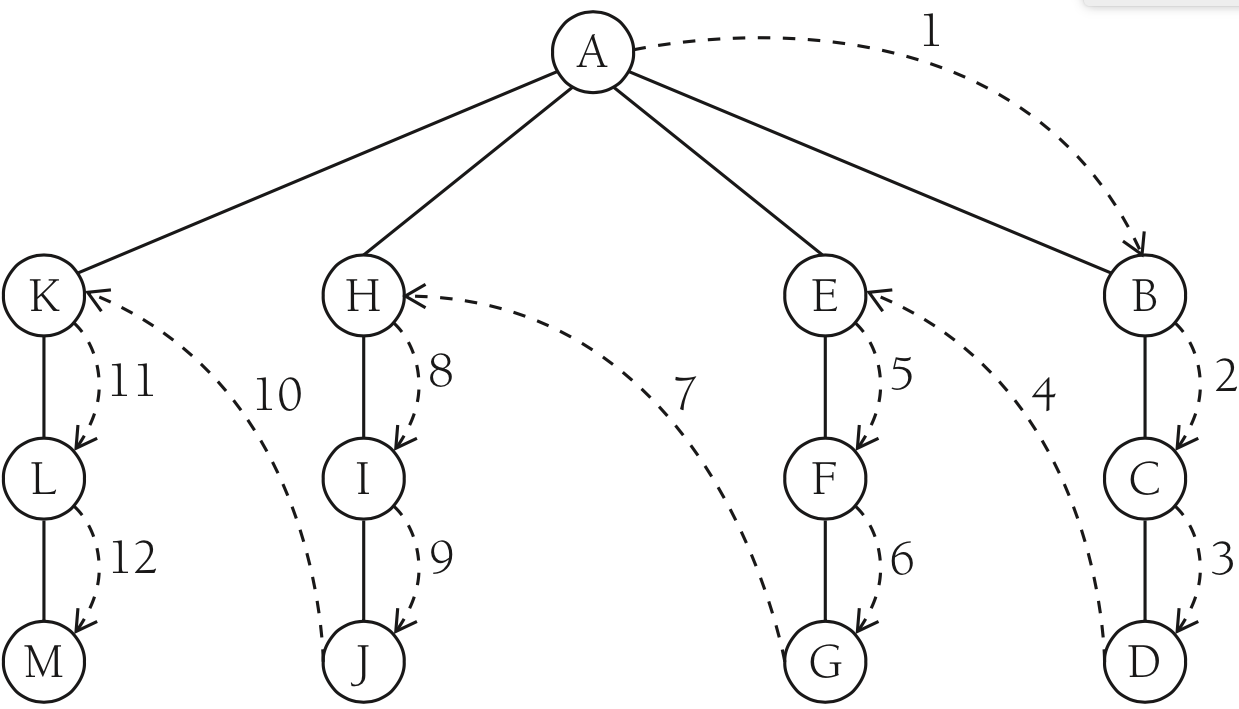
\includegraphics[scale=0.2]{figuras/algWorks2}
	\caption{Depth-First Search.}
	\label{fig:algWorks2}
\end{figure}






%As can be visualized, a stack is used to store all affected elements, see Algorithm~\ref{alg:death1} line 2, \ding{182}. In line 3 a generic KDM element is defined. While \textit{seg} is non-empty, a node is chosen for expansion (line 4). %For fact edges, the dependency of the edge on the particular fact that caused its creation is then recorded (lines 14- 16)





%\begin{algorithm}[h]
%     \SetAlgoLined
%     \KwIn{KDMEntity kdmElement, Segment segment, KDMModel model}
%     \KwOut{All affected metaclasses}
%     \Begin{
%   $ Stack stack \longleftarrow \{\}$\;
%   KDMEntity elementToVerify\;
%     \ForEach{$seg$ in $segment$} {
%	\eIf{seg.getOwnedElements() != null}{
%			\If{seg.getNextSiblind() != null}{
%				$elementToVerify \longleftarrow seg.getNextSiblind()$\;
%		\If{\ding{182} isAffected(elementToVerify, kdmElement, model)}{
%					stack.push(elementToVerify)\;
%					$seg \longleftarrow  seg.getFirstChild()$\;
%				}				
%			}		
%	
%	}{ $seg \longleftarrow seg.getNextSiblind()$\;
%		\If{seg = null \&\& stack.isEmpty()}{
%			// return to the parent's level
%		}
%	}
%     }
%	\ding{184} \Return{stack}
%     }
%     \caption{Depth-First Search Algorithm.}
%     \label{alg:death1}
%   \end{algorithm}
%
%\begin{algorithm}[h]
%     \SetAlgoLined
%     \KwIn{KDMEntity kdmElement, KDMModel model, KDMEntity e}
%     \KwOut{true or false}
%     \Begin{
%     	\If{ (e = AbstractUIElement) or (e = AbstractStructureElement) or (e = BuildResource) or (e = AbstractPlatformElement) or (e = AbstractConceptualElement) or (e = AbstractEventElement)
%				} {
%					     \ForEach{$elements$ in $e.getImplementation()$} {
%					\If{ elements = ele} {
%					\Return{true}
%					}
%					}				
%				}
%\uElseIf{ e = AbstractDataElement
%				} {
%					     \ForEach{$elements$ in $elementToV.getDataRelation()$} {
%					\If{ elements = elementToVerify} {
%					\Return{true}
%					}
%					}				
%				}
%	...
%     }
%     \caption{isAffected Algorithm}
%     \label{alg:death}
%   \end{algorithm}

%As every element, except the Segment, is connected somehow it is necessary to iterate throughout them, line 4 of Algorithm~\ref{alg:death} illustrates this iteration. After, the method \texttt{isAffected(...)} is called to verify if the element is affected.  If the condition in line 8 evaluates to true, then the element is pushed into the stack defined in line 2. Finally, in line 20 the stack is returned with all affected elements, see Algorithm~\ref{alg:death} \ding{184}. 

\subsection{Apply Refactoring} % (fold)
\label{sub:apply_refactoring}

In the step [B] the engineer must apply the refactoring. A natural way of implementing refactoring in models is by means of \textit{in-place transformations}\footnote{We have devised a repository where a set of \textit{in-place transformations} (i.e., refactoring) is available. The repository can be accessed in www.site.com.br. It aims is to share refactoring to be applied into KDM's instances.} as describe in Section~\ref{sec:background}. %This kind of transformations are used for rewriting a model by creating, deleting, and updating elements in the input model, e.g., in a KDM's instance. 
Going into more details, applying these transformations/refactoring into a KDM's instance can introduce incompatibilities and inconsistencies which can not be easily resolved. In fact, we can classified these transformations by their corrupting or non-corrupting effects:%\cite{towardssynchronizing07}:

\begin{itemize}
\item \textit{non-breaking changes}: changes which do not break the KDM's instance - for instance, the refactoring rename;

\item \textit{breaking and resolvable changes automatically}: changes which do break the KDM instance, but can be resolved by automatic means - for instance, apply the refactoring \textit{move class, extract class, push meta-attributes}, etc;

\item \textit{breaking and unresolvable changes automatically}: changes which do break the KDM instance and can not be resolved automatically - for instance, when manual interventions are needed.
%
\end{itemize} 
% In the context of this paper, we are only considering the \textit{non-breaking changes} and \textit{breaking and resolvable changes automatically}. 
%
These transformations can be performed by means of rule-based languages. Our approach uses ATL Transformation Language (ATL). The main advantage of using one ATL is that the transformation logic can be expressed at a high level of abstraction thus enhancing maintainability and understandability. 

To express a transformation in our approach, the user must specify mapping rules that describe how KDM's elements model can be refactored. Further, the users should inform some input parameters that should be properly instantiated. For example, considering the refactoring \textit{Move Class}, an ATL transformation that could perform this task is depicted in Figure~\ref{fig:ATLRefactoring}.








%A natural way of implementing refactoring in models is by means of \textit{in-place transformations}\footnote{The term \textit{in-place transformations} stands for transformations rewriting a model, as opposed to producing a model from scratch which is done by \textit{out-place transformations}.} 

%\textit{In-place transformations} can be described in many ways. Rule-based descriptions are elegant and easy to understand. Such descriptions have declarative model rewriting rules as their primitive building blocks. A rule consist of a \textit{Left Hand Side} (LHS) pattern that is matched against a model. If a match is found, this pattern is updated in the model, based on what is specified in the \textit{Right Hand Side} (RHS) of the rule.

 %We have devised a repository where a set of \textit{in-place transformations} (i.e., refactoring) is available\footnote{The repository can be accessed in www.site.com.br. It aims is to share refactoring to be applied into KDM's instances}. All the \textit{in-place transformations} can be written either in ATL Transformation Language (ATL) or Query/View/Transformation (QVT). Due space limitation this repository is not shown. However, the reader should keep in mind from where we get the in-place transformations. Considering again the running example presented in Section~\ref{sec:motivation_and_running_example}, where the \textit{Move Class} refactoring must be applied. Then the engineer must browser our repository and choose the refactoring \textit{Move Class}.

\begin{figure}[h]
	\centering
	% Requires \usepackage{graphicx}
	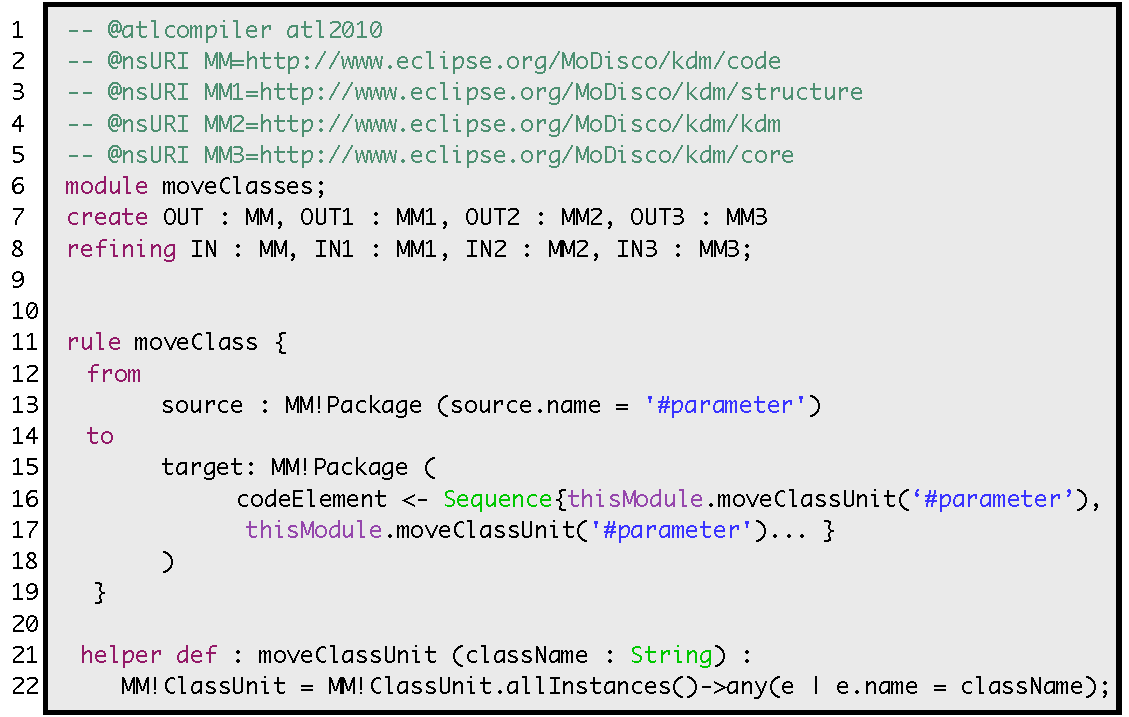
\includegraphics[scale=0.47]{figuras/ATLTRansformationLanguage}
	\caption{Chunk of code in ATL to perform the refactoring \textit{Move Class}.}
	\label{fig:ATLRefactoring}
\end{figure}


By inspecting this transformation/refactoring we can see important informations. For instance, lines 1 to 5 illustrate which KDM's level/packages are be affected by this transformation.  After, in line 6 it is possible to see the name of our transformation, \texttt{moveClasses}. Lines 7 and 8 represent the output and input models that conform to the KDM, e.g., the model used during the transformation/refactoring. 
%
With the \texttt{refining} mode (see Line 8 of Figure~\ref{fig:ATLRefactoring}), the ATL engine can focus on the ATL code dedicated to the generation of modified target elements. Other KDM elements (e.g. those that remain unchanged) are implicitly processed by the ATL engine.

%The keyword \texttt{refining} means informs to the ATL engine that  to the ATL engine that this transformation is \textit{in-place}

Line 11 a matched rule is defined. In fact, this rule represents the refactoring \textit{Move Class}. Occurrences of the input pattern may be filtered by introducing a \textit{guard}, a boolean condition that KDM model must satisfy (e.g., line 13). Lines 14 though 19 the refactoring \textit{Move Class} is actually defined. As can be seen, we are moving a set of \texttt{ClassUnit} by means of the helper (defined in lines 21 and 22). 
Almost all refactorings need some input parameters that should be properly instantiated by the user. For instance, consider the chuck of code written in ATL depicted in Figure~\ref{fig:ATLRefactoring}, lines 13, 16, and 17 (\texttt{\#parameter}). Therefore, before to apply the refactoring, the user should set the parameters. Considering our running example (depicted in Figure~\ref{fig:system}) the parameters would be: \texttt{Model}, \texttt{Student}, and \texttt{Instructor}, respectively. Afterward, this ATL is ready to be applied into a KDM instance.


%It is important to highlight that this chuck of code in written in ATL is not total functional - the engineer should set the parameters (\texttt{\#parameter}) 

%Refactorings are implemented by specifying its actions that have to be executed for applying the change. Most of them need also some input parameters that should be properly instantiated by the user. For instance, consider the chuck of code written in ATL depicted in Figure~\ref{fig:ATLRefactoring} 

\subsection{Propagate Changes} % (fold)
\label{sub:apply_refactoring}

In this step, all propagating is implemented. In fact, this step is performed along with the step [B].

In the step [C] all the changes, that where resulted by the refactoring  performed in step [b] need be propagate into all KDM's levels/package.  




%\section{Refactoring Meta-model}~\label{sec:refactoring_metamodel}
%	%As stated beforeKDM does not provides suitable meta-classes to apply refactorings. 

Previous work on model refactoring focused on UML models (Biermann et al., 2006; Mens, 2005; Mens et al., 2007). However, when these UML models are refactored, the respective changes have to be propagated into either different artefacts or other levels, i.e., distinct models; otherwise, the system represented in model is no longer consistent with the model. As the KDM is a meta-model that aims to model all of a given system, it allows the propagation and traceability of changes after the application of a refactoring.


Previous works are related to static context - within a static context, refactoring of model will probably never cause any problems. But many models evolve in time: elements are renamed, layer are created, relationship are changed, references are re-targeted and classes are inlined or extracted in order to create or collapse inheritance hierarchies or just to improve the model - in short: the model is refactored. Regarding only UML models, applying these refactorings is well understood and implemented in several ways. However, in the context of the KDM models there is none research in this area. Therefore, we claim that research must to be done in this direction. The problem is usually caused by the strong interconnection between KDM's packages, all KDM's packages are connected somehow (see Section~\ref{sec:background}), e.g., the package Structure uses meta-classes from package Code, the package Code uses meta-classes from package core, etc. Therefore, if any meta-class is just referencing the refactored model meta-class, after refactoring, this reference can be unset. Hence, the KDM model is invalid because of inconsistencies between its packages. 


Therefore in this section we propose an approach to assist the propagation of refactoring into KDM's packages. Our approach starts with Fowler`s definition of each refactoring. As these definitions were introduced for the refactoring of (object oriented) code, we adapt the definitions for KDM model refactorings. Subsequently we investigate how the changes affect the KDM's packages. Herein we consider different aspects concerning the KDM's packages. For instance, depending on the meta-class the refactoring may cause minor or major changes to be propagated into other packages.

In order to explain the propagation of changes in KDM in this section a set of examples is used. The first system is presented in Figure~\ref{fig:system} (A).As noted in Figure~\ref{fig:system} (A) two layers have been defined. The first one is ``View'' and the second layer is ``Controller''. Inside of each layer there is one package. The relationships ``GUI inside View'' and ``CTR inside Controller'' mean that ``GUI'' and ``CTR'' are in container ``View'' and ``Controller'', respectively or in some sub-container of  ``View'' and ``Controller'', transitively. In the same way, the relationship ``StudentGUI inside GUI'' means that ``StudentGUI'' is in container ``GUI'' or in some sub-container of ``GUI''. For relationships, let R' be the corresponding aggregated relationship, which represents the number summing all primitive relationships, i.e., ``Calls'', ``Creates'', ``Extends'', etc. 

The corresponding, though simplified KDM instance of Figure~\ref{fig:system} (A) is depicted in Figure~\ref{fig:system} (B). It illustrates a KDM instance as a UML object diagram for the sake of simplicity, note that this diagram represents the system in  as a tree of nodes containing some KDM`s meta-classes. Analysing both figures it is evident that each element presented in Figure~\ref{fig:system} (A) has a meta-class in KDM to represent it. For instance, the layers are represented in KDM using the meta-class Layer. Each primitive relationship has also a meta-class in KDM. The meta-class ``AggregatedRelationship'' represents a set of primitive KDM relationships. 

In order to increase the modularity of the system consider that the engineer has chosen to apply refactoring extract package to create a package model. In Figure~\ref{fig:atl} is depicted a chunk of code written in ATL responsible to perform the refactoring extract package.

Firstly, an instance of meta-class Package must be created. Then the name of it must be defined. After the creation of this package one must group the instance of all classes that will be moved to the new package. The refactoring at this point can be considered complete for the package code of KDM. However, now it is necessary to propagate all the changes to other KDM's packages. In Figure~\ref{fig:atl2} is presented a chunk of code responsible for performing the propagation of changes. As can be seen, it is necessary to create an instance of the meta-class Layer, set its name to ``Controller'', see lines X-Y of Figure~\ref{fig:atl2}. Then, the association ``implementation'' of ``Layer'' earlier created need to be specified. In this point it is important to visualise that this association refers to the extracted package, i.e., the package created earlier. Further, it is necessary to create an instance of meta-class AggregatedRelationship. This meta-class has a meta-attribute, ``density'' and a set of association that need to be propagated. The part of the source code responsible to create an AggregatedRelationship is presented in lines 17-23 of Figure~\ref{fig:atl2}. The helper illustrated in lines X-Y represents that the meta-attribute ``density'' is updated always that a new relationship is identified.




We can divide the propagation in three the possible scenarios. The first scenario is presented in Figure X. As noted 



Suppose the system presented in Figure~\ref{fig:system}. This system was developed using the architectural style Model-View-Controller.




%!TEX root = /Users/rafaeldurelli/Dropbox/Artigos Elaborados/KDM propagation_2015/sbes_2015_kdm_propagation/sbes2015_kdm_propagation.tex

A case study showing that our approach can be used to support the change propagation in KDM models is presented in this section. Throughout this case study we have used the described running example, i.e., we applied our three step approach in LabSys.
The object of this study is our proposed approach to propagate changes, and the purpose of this study is to evaluate the effectiveness of it. Taking into account the object and purpose of the study, we defined one research question:
\textit{ \textbf{RQ$_{caseStudy}$}: Given a set of refactoring (\textit{Extract Class}, \textit{Move Class}, \textit{Extract Layer} and \textit{Remove Class}),
can the proposed approach propagate all the changes effectively throughout KDM views}?


To assess the effectiveness of the proposed approach through the \textbf{RQ$_{caseStudy}$}, we use some oracles. As each refactoring has its own characteristics and modifies specific KDM model elements, it is possible to predict all the expected changes in other KDM views. So, considering our set of developed refactorings, we had to develop some oracles for each refactoring. The complete oracle can be seen at www.mudar.com.br.

The execution of this case study was assisted by our Eclipse plug-in that we developed to support the proposed approach. As stated in Section~\ref{sec:the_approach} the proposed approach uses as input two KDM instance, one representing the LabSys, and one conforming the refactored LabSys. Therefore, firstly we adopted a reverse engineering to transform the LabSys source-code into a KDM instance. We used MoDisco\cite{Brunele20141012}, which is a framework that get as input java source-code and then return as output a KDM instance. Currently, MoDisco only generates the KDM \texttt{Code package}, other KDM packages are extremely important to evaluate our approach. Therefore, we manually instantiated the followings KDM packages: \texttt{Structure Package}, \texttt{Data Package}, and \texttt{Conceptual Package}. After applying LabSys to MoDisco we gathered a KDM instance that contains 29,444 number of model instances (in this context KDM meta-classes' instances in the model). %The memory used on hard drive disk after XMI serialization is 5.66 MB. 

After that, we applied each refactoring and generated another KDM instances, i.e, this new KDM instance represent a new LabSys version, the refactored one. Then, we applied the step [B] of our approach - then a diff between the original KDM instance and the refactored one was performed. Finally, we applied the step [C] in order to propagate all the changes throughout KDM views. These steps were executed four times, i.e, for each chosen KDM refactoring all these step was performed.

As stated earlier, LabSys contains some flaws. More specifically, one an evident problem in this system is the presence of the ClassUnits \texttt{Student} and \texttt{Instructor} in the VIEW package, these ClassUnits should be allocated in the MODEL package. Another problem is that the ClassUnits \texttt{Laboratory} is doing work should be done by two ClassUnits. Similarly, by inspecting the LabSys instance we could notice that there is a ClassUnit that is no longer used, it does not contains any relationship with another ClassUnit. Finally, the \texttt{MODEL} Layer should also be extracted as it also contains internals elements responsible to deal with database information. 

In order to solve these flaws we selected selected three class-level refactorings (\textit{Extract Class}, \textit{Move Class} and \textit{Remove Class}) and one layer-level. The class-level refactorings are the conventional and well known Fowler's~\cite{refactImpro} refactorings easily found on literature. The conceptual order of applying these refactorings are botton-up, i.e., from lower level elements to higher level ones. For example, when you move classes from one package to another, business rules representing those classes should also be moved to other scenarios.

The refactoring  layer-level was intend to investigate top-down propagations, so, we decided to apply the \textit{Extract Layer} refactoring. The goal of this refactoring is the extraction of responsibilities from one layer and the moving of them to a recently created one. In this case, the propagation is from top to down, because it is necessary to propagate changes to lower level elements, such as Packages and ClassUnits, for example. 

It is important to highlight that all these KDM refactoring were devised in ATL. However, due space limitation only the refactoring \textit{Move Class} is depicted and explained.

\begin{figure}[h]
	\centering
	% Requires \usepackage{graphicx}
	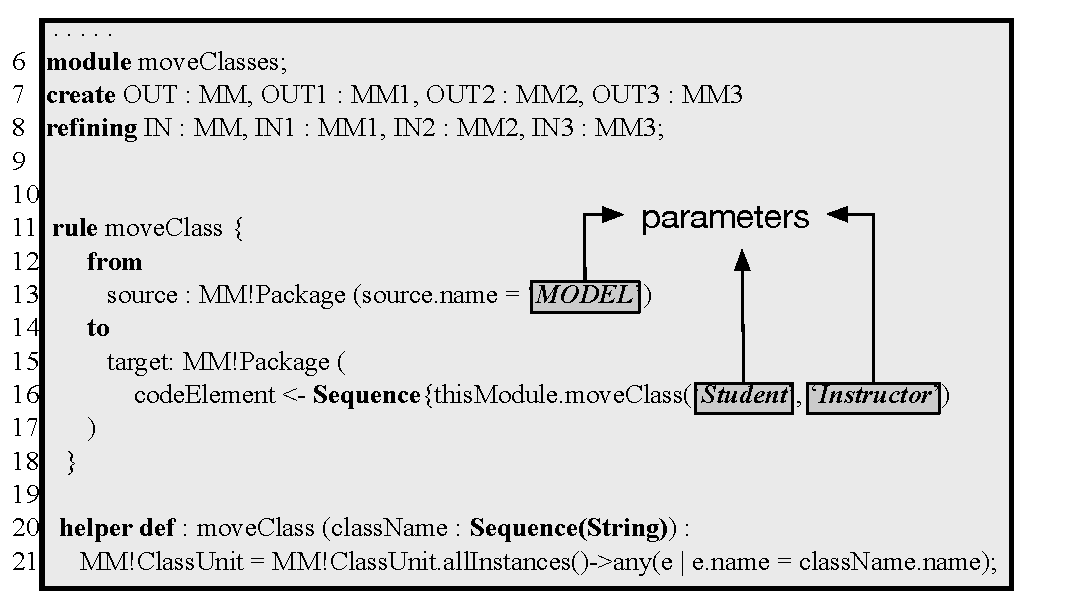
\includegraphics[scale=0.516]{figuras/NovoMoveClassFormatted}
	\caption{Snippet of ATL to perform the refactoring \textit{Move Class}.}
	\label{fig:ATLRefactoring}
\end{figure}

These KDM refactorings need some parameters that should be properly informed before to start our three step approach. For instance, considering the refactoring illustrated in Figure~\ref{fig:ATLRefactoring} lines 13 and 16 three parameters specified, i.e, the source Package (\texttt{MODEL}) and two ClassUnit's instances (\texttt{Student} and \texttt{Instructor}) to be moved were specified. %that he(she) would like to move.
After specifying these parameters the ATL is ready to be applied into a KDM instance.


All refactorings were applied completely automatically by means of our devised plug-in, we just needed to specify all parameters. To deal with refactorings that go into infinite loops, we set three minutes timeout interval. 
%More specifically, 
We applied the \textit{Extract Class} to the ClassUnit \texttt{Laboratory}; we applied the \textit{Move Class} to two ClassUnit's instances (\texttt{Student} and \texttt{Instructor}); we applied the \textit{Extract Layer} to the \texttt{MODEL} Layer that contains internals elements to deal with database information; finally we applied the \textit{Remove Class} to a ClassUnit that was no longer used in LabSys.

The effect of applying these four KDM refactoring will turn the KDM instance inconsistent. For instance, considering the KDM refactoring \textit{Move Class} depicted in Figure~\ref{fig:ATLRefactoring} the ``density'' value will turn wrong, i.e., AggregationRelationShip between
the Layer VIEW and the Layer CONTROLLER would
change from 4 to 2 - once the primitives relationships Creates
and Extends would no longer exist from the package VIEW
to the package CONTROLLER. In the same way, the result of \textit{Move Class} refactoring should also update the density between the Layer
MODEL and CONTROLLER, instead of 2 it should be 4, as
Creates and Extends were also moved along with its
ClassUnits, \texttt{Student} and \texttt{Instructor}. Concerning to the
Conceptual View, the RuleUnit \textit{CheckFreeHours} that is associated with
\texttt{Instructor} should also be moved to ScenarioUnit \textit{RegisterStaff}. Others desynchronization would also arise after applying all described KDM refactorings. 

%moving these ClassUnits will turn the KDM instance inconsistent, because the ``density'' value will turn wrong, i.e., AggregationRelationShip between the Layer VIEW and the Layer CONTROLLER would change from 4 to 2 - once the primitives relationships Creates and Extends would no longer exist from the package VIEW to the package CONTROLLER. In the same way, the result of \textit{Move Class} refactoring should also update the density between the Layer MODEL and CONTROLLER, instead of 2 it should be 4, as Creates and Extends were also moved along with its ClassUnits, \texttt{Student} and \texttt{Instructor}. Concerning to the Conceptual View, the RuleUnit \textit{CheckFreeHours} that is associated with \texttt{Instructor} should also be moved to ScenarioUnit \textit{RegisterStaff}.
After applied all refactorings we verify whether them were successfully propagate throughout KDM views, i.e., if the intended refactoring could be performed and if all the expected propagations were generated on the KDM model. 
Based on a set of oracle it was possible to verify if all refactoring were successfully propagated throughout KDM models. Using these information gathered we can draw conclusion and answer the \textbf{RQ$_{caseStudy}$}. Table~\ref{tab:prop} summaries the results related to each refactoring applied and its respective propagations. In this table there are two abbreviations: (i) ``P.C?" (``Propagation Corrected?") and (ii) ``N.A" (``Not Applied"). This table also depicts the propagation regarding to the followings KDM packages: \texttt{Structure Package}, \texttt{Data Package}, and \texttt{Conceptual Package}. 

All the changes were effectively propagated throughout KDM views. Which means that in this case our approach could automatically execute truly relevant propagation in all KDM views when dealing with the chosen refactorings. Observing globally the data in Table~\ref{tab:prop} we can claim that the use of our approach in the context of these refactorings has been satisfactory. The data also show that our approach it is able to propagate changes in KDM view in an effective way and it also yields concise propagation of changes. Thereby, the \textbf{RQ$_{caseStudy}$} can be answered as true, that is, the proposed approach can propagate changes effectively throughout KDM views.

\begin{table*}
\centering
\caption{Propagations for the refactorings: Extract Class, Extract Layer, Move Class, and Remove Class\label{tab:prop}}
{\footnotesize{}}%
\setlength{\tabcolsep}{0.0em}
{\renewcommand{\arraystretch}{0.5}
\begin{tabular}{|l|>{\raggedright}p{7cm}|c|l|>{\raggedright}p{7cm}|c|}
\hline 
\textbf{\footnotesize{\cellcolor{gray!40}Refactoring}} & \textbf{\footnotesize{\cellcolor{gray!40}Extract Class}} & \textbf{\footnotesize{\cellcolor{gray!40}P.C?}} & \textbf{\footnotesize{\cellcolor{gray!40}Refactoring}} & \textbf{\footnotesize{\cellcolor{gray!40}Extract Layer}} & \textbf{\footnotesize{\cellcolor{gray!40}P.C?}}\tabularnewline
\hline 
\hline 
\multirow{4}{*}{{\footnotesize{Code}}} & {\footnotesize{Create an instance of ClassUnit that represent the
new Class}} & {\footnotesize{Yes}} & \multirow{2}{*}{{\footnotesize{Code}}} & {\footnotesize{Create an instance of Package}} & {\footnotesize{Yes}}\tabularnewline
\cline{2-3} \cline{5-6} 
 & {\footnotesize{Move all StorableUnits to the new ClassUnit}} & {\footnotesize{Yes}} &  & {\footnotesize{Move a set of selected ClassUnits from a Package to the
new Package}} & {\footnotesize{Yes}}\tabularnewline
\cline{2-6} 
 & {\footnotesize{Move all MethodUnit to the new ClassUnit}} & {\footnotesize{Yes}} & \multirow{4}{*}{{\footnotesize{Structure}}} & {\footnotesize{Create an instance of Layer}} & {\footnotesize{Yes}}\tabularnewline
\cline{2-3} \cline{5-6} 
 & {\footnotesize{Create an intance of HasType, which represent an association
between the new ClassUnit and the old ClassUnit}} & {\footnotesize{Yes}} &  & {\footnotesize{Create an instance of AggregationRelationship between
the new Layer and the old one}} & {\footnotesize{Yes}}\tabularnewline
\cline{1-3} \cline{5-6} 
{\footnotesize{Structure }} & {\footnotesize{N. A}} & {\footnotesize{N.A}} &  & {\footnotesize{Associate the new Layer by means of the association
implementation with the new Package}} & {\footnotesize{Yes}}\tabularnewline
\cline{1-3} \cline{5-6} 
\multirow{3}{*}{{\footnotesize{Data }}} & {\footnotesize{Create a instance of RelationalTable owning the name
of the new ClassUnit}} & {\footnotesize{Yes}} &  & {\footnotesize{Summing up all primitive relationship to compute the
meta-attribute density}} & {\footnotesize{Yes}}\tabularnewline
\cline{2-6} 
 & {\footnotesize{For each StorableUnit it is necessary to create a ItemUnit,
which represent the RelationaTable columns.}} & {\footnotesize{Yes}} & {\footnotesize{Data}} & {\footnotesize{N. A}} & {\footnotesize{N. A}}\tabularnewline
\cline{2-6} 
 & {\footnotesize{Create an instance of UniqueKey that represent the
primary key of the RelationalTable.}} & {\footnotesize{Yes}} & \multirow{2}{*}{{\footnotesize{Conceptual}}} & {\footnotesize{If the moved classes are associated to any conceptual
elements by means of the association implementation these conceptual
elements should be moved to a correspondent associated element of
the target Package.}} & \multirow{2}{*}{{\footnotesize{Yes}}}\tabularnewline
\cline{1-3} 
{\footnotesize{Conceptual}} & {\footnotesize{N. A}} & {\footnotesize{N. A}} &  &  & \tabularnewline
\hline 
\textbf{{\footnotesize{\cellcolor{gray!40}Refactoring}}} & {\textbf{\footnotesize{\cellcolor{gray!40}Move Class}}} & {\textbf{\footnotesize{\cellcolor{gray!40}P.C?}}} & {\textbf{\footnotesize{\cellcolor{gray!40}Refactoring}}} & {\textbf{\footnotesize{\cellcolor{gray!40}Remove Class}}} & {\textbf{\footnotesize{\cellcolor{gray!40}P.C?}}}\tabularnewline
\hline 
{\footnotesize{Code}} & {\footnotesize{Move an specific ClassUnti from a source Package to
a target Package}} & {\footnotesize{Yes}} & {\footnotesize{Code}} & {\footnotesize{Delete the selected instance of a ClassUnit}} & {\footnotesize{Yes}}\tabularnewline
\hline 
{\footnotesize{Structure}} & {\footnotesize{If the target Package is associated to an architectural
elements by means of the association implementation the value of meta-attribute
named density should be propagated}} & {\footnotesize{Yes}} & {\footnotesize{Structure}} & {\footnotesize{If the removed ClassUnit was contained into a specific
Structure element then summing up all primitive relationship and overwrite
the meta-attribute density}} & {\footnotesize{Yes}}\tabularnewline
\hline 
{\footnotesize{Data}} & {\footnotesize{N. A}} & {\footnotesize{N. A}} & {\footnotesize{Data}} & {\footnotesize{if the removed ClassUnit was associated with an instance
of RelationalTable, then it should also be removed}} & {\footnotesize{Yes}}\tabularnewline
\hline 
{\footnotesize{Conceptual}} & {\footnotesize{If the moved class is associated to any conceptual
elements by means of the association implementation this conceptual
elements should be moved to a correspondent associated element of
the target Package.}} & {\footnotesize{Yes}} & {\footnotesize{Conceptual}} & {\footnotesize{if the removed ClassUnit is associated to any conceptual
elements by means of the association implementation these conceptual
elements should be removed}} & {\footnotesize{Yes}}\tabularnewline
\hline 
\end{tabular}}
\end{table*}


%%!TEX root = /Users/rafaeldurelli/Dropbox/Artigos Elaborados/KDM propagation_2015/sbes_2015_kdm_propagation/sbes2015_kdm_propagation.tex
\section{Proof-of-Concept Implementation}

We devised a Eclipse plug-in named Modernization-Integrated Environment (MIE) which is split in three layers, as follows: (\textit{i}) Core Framework, (\textit{ii}) Tool Core, and (\textit{iii}) Graphical User Interface (GUI). This plugin was devised on the top of the Eclipse Platform; The first layer we used both Java and Groovy as programming language. Moreover, the Core Framework layer contains a set of Eclipse plug-ins on which our environment is based on, such as MoDisco and Eclipse Modeling Framework (EMF)\footnote{http://www.eclipse.org/modeling/emf/}. We used MoDisco\footnote{http://www.eclipse.org/MoDisco/} once it is an extensible framework to develop model-driven tools to support use-cases of existing software modernization and provides an Application Programming Interface - (API) to easily access the KDM model. Also, EMF was used to load and navigate KDM models that were generated with MoDisco. The second layer, the Tool Core, is where the steps presented in Section~\ref{sec:the_approach} were implemented. Herein, we work intensively with KDM models, which are XML files. Therefore, we use XPath to handle those types of files, to mine the affected metaclasses, ATL to perform the refactoring and to propagated them. Finally, the third layer is the Graphical User Interface (GUI) that consists of a set of SWT windows with several options to perform the refactorings based on the KDM model.




% Figure~\ref{fig:architecture} depicts the architecture of this environment. As shown in this figure, the first layer is the Core Framework. This layer represents that  we devised the  environment on the top of the Eclipse Platform. In this layer it is also possible to see that we used both Java and Groovy as programming language. Moreover, this layer contains Eclipse Plugins on which our environment is based on, such as MoDisco and EMF. We used MoDisco\footnote{http://www.eclipse.org/MoDisco/} once it is an extensible framework to develop model-driven tools to support use-cases of existing software modernization and provides an Application Programming Interface - (API) to easily access the KDM model. Also, Eclipse Modeling Framework (EMF)\footnote{http://www.eclipse.org/modeling/emf/} was used to load and navigate KDM models that were generated with MoDisco. 

%\begin{figure}[!ht]
%\centering
  % Requires \usepackage{graphicx}
 % \includegraphics[scale=0.6]{FIGURAS_DA_REFATORACAO/Arquitetura}
%\caption{Architecture of the proof-of-concept implementation.}
%\label{fig:architecture}
%\end{figure}  

%The second layer, the Tool Core, is where all refactorings provided by our environment were implemented. It works intensively with KDM models, which are XML files. Therefore, we use Groovy to handle those types of files because of the simplicity of its syntax and fully integrated with Java.  After the engineer to realize all refactorings a forward engineering must be carried out - then the source code of the refactored target system is generated. Finally, the top layer is the Graphical User Interface (GUI) that consists of a set of SWT windows with several options to perform the refactorings based on the KDM model.

%!TEX root = /Users/rafaeldurelli/Dropbox/Artigos Elaborados/KDM propagation_2015/sbes_2015_kdm_propagation/sbes2015_kdm_propagation.tex

This section describes the experiment used to evaluate the effectiveness of our MDI Algorithm, step [B] of our approach. We compared its result manually in order to verify its correctness. %The second experiment is referred as ``Propagation Study'' and was planned to evaluated the correctness of the propagation given a set of refactorings. 
In addition, we worked out one research question, as follows:
%
%Moreover, this experiment also evaluate the devised Eclipse plug-in, which was earlier described. Specifically, we investigate the following research questions:
%
\textit{\textbf{RQ$_{experiment}$}: Given some specific elements to be refactored, is the DI Algorithm able to identify correctly all the dependent KDM elements?}

%\textbf{RQ$_{2}$}: Given a specific refactoring R, are all dependent elements identified in the oracle correctly refactored?
 
%To evaluate these questions we we carried out two steps. Firstly, we have evaluated our mining algorithm. Therefore, we have compared its result with an oracle in order to verify its correctness. Similarly, we have evaluated the correctness of a set of refactorings. Thus,  we have also compared its results to the same oracle mentioned previously.

\subsection{Goal Definiton}\label{sec:goal_definition}

We use the organization proposed by the Goal/Question/Metric (GQM) paradigm, it describes experimental goals in five parts, as follows:
%
%\begin{itemize}
%
%\item \textbf{object of study:} the object of study is our approach; 
%
%\item \textbf{purpose:} the purpose of this experiment is to evaluate the effectiveness of our mining approach; %The experiment provides insight into how much effective can be our mining approach. It is also expected that the experimental results can be used to evaluate the impact of idenfiforking the execution of mutant methods in their own threads and weakly killing them have on the performance.
%
%\item \textbf{perspective:} this experiment is run from the standpoint of a researcher;
%
%\item \textbf{quality focus:} the primary effect under investigation is the precision and recall after applying the mining algorithm; 
%
%\item  \textbf{context:} this experiment was carried out using Eclipse 4.3.2 on a 2.5 GHz Intel Core i5 with 8GB of physical memory running Mac OS X 10.9.2.
%\end{itemize}
%
(\textit{i}) \textbf{object of study:} the object of study is our MDI Algorithm; (\textit{ii}) \textbf{purpose:} the purpose of this experiment is to evaluate the effectiveness of our MDI Algorithm; (\textit{iii}) \textbf{perspective:} this experiment is run from the standpoint of a researcher; (\textit{iv}) \textbf{quality focus:} the primary effect under investigation is the precision and recall after applying the MDI Algorithm; (\textit{v}) \textbf{context:} this experiment was carried out using Eclipse 4.3.2 on a 2.5 GHz Intel Core i5 with 8GB of physical memory running Mac OS X 10.9.2.

The experiment can be summarized using Wohlin et al.'s template~\cite{Wohlin} as follows: 

\textbf{Analyze} the effectiveness of our MDI Algorithm

\textbf{for the purpose of} evaluation

\textbf{with respect to} precision and recall

\textbf{from the point of view of} the researcher

\textbf{in the context of} a subject program. 

%The experiment can be defined as: \textbf{Analyze} the effectiveness of our mining algorithm, \textbf{for the purpose of} evaluation, \textbf{with respect to} precision and recall, \textbf{from the point of view of} the researcher, \textbf{in the context of} a subject program. 

\subsection{Effectiveness Analysis}\label{hypothesis_formulation}	

We present an effectiveness analysis to determine the recall and precision of our approach. Thus, we applied our MDI Algorithm in one system and we performed a manual analysis to verify the effectiveness of our MDI Algorithm. This analysis employs two metrics: recall and precision, which are described below:

\begin{itemize}
\item Precision is the ratio of the number of true positives retrieved to the total number of irrelevant and relevant KDM elements retrieved. It is usually expressed as a percentage, see equation 1.
\end{itemize}
%In order to accomplish our goal, we explored the formalization of our research question into hypotheses so that statistical tests can be performed. The hypotheses are shown in Table~\ref{tab:hypotheses}. There are two variables shown on each table: `P' and `R'. `P' stands for Precision which is the ratio of the number of true positives retrieved/identified to the total number of irrelevant and relevant code elements retrieved/propagated. It is usually expressed as a percentage, see equation 1. `R' denotes Recall which is the ratio of the number of true positives retrieved/propagated to the total number of relevant code elements in the source code. It is usually expressed as a percentage, see equation 2. 

%\begin{table}[h]
%\centering
%\caption{Hypotheses for the Mining Study\label{tab:hypotheses}}
%~~\\
%\begin{tabularx}{
%.46\textwidth}{|c|X|}
%There is no difference between using our tool and using an ad-hoc reuse process in terms of productivity (time) to couple sucessfully a CF with an application.
%\hline \cellcolor[gray]{\shadow} H$_0$ & \footnotesize{ There is no difference in pattern recognition before and after to apply our mining affected metaclasses algorithm into the KDM model (measured in terms of the metric precision (P) and recall (R)) which can be formalized as: 

%\textbf{H$_{0}$: $\mu_{P_{Bf}} = \mu_{P_{Af}}$ and $\mu_{R_{Bf}} = \mu_{R_{Af}}$}}
%\\
%\hline \cellcolor[gray]{\shadow} H$_1$ & \footnotesize{There is a significant difference in pattern recognition before and after to apply our mining affected metaclasses algorithm into the KDM model (measured in terms of the metric precision (P) and recall (R)) which can be formalized as: 

%\textbf{H$_{1}$: $\mu_{P_{Bf}} \neq \mu_{P_{Af}}$ and $\mu_{R_{Bf}} \neq \mu_{R_{Af}}$}}
%\\
%\hline
%\end{tabularx}
%\end{table}

%\begin{table}[h]
%\centering
%\caption{Hypotheses for the Propagation Study\label{tab:hypotheses}}
%~~\\
%\begin{tabularx}{
%.46\textwidth}{|c|X|}
%There is no difference between using our tool and using an ad-hoc reuse process in terms of productivity (time) to couple sucessfully a CF with an application.
%\hline \cellcolor[gray]{\shadow} H$_0$ & \footnotesize{ There is no difference in propagation of changes before and after to apply a refactoring into the KDM model (measured in terms of the metric precision (P) and recall (R)) which can be formalized as: 

%\textbf{H$_{0}$: $\mu_{P_{Bf}} = \mu_{P_{Af}}$ and $\mu_{R_{Bf}} = \mu_{R_{Af}}$}}
%\\
%\hline \cellcolor[gray]{\shadow} H$_1$ & \footnotesize{There is a significant difference in propagation of changes before and after to apply a refactoring into the KDM model (measured in terms of the metric precision (P) and recall (R)) which can be formalized as:  
%
%\textbf{H$_{1}$: $\mu_{P_{Bf}} \neq \mu_{P_{Af}}$ and $\mu_{R_{Bf}} \neq \mu_{R_{Af}}$}}
%\\
%\hline
%\end{tabularx}
%\end{table}

%\textbf{Null hypothesis, H$_{0}$}: There is no difference in pattern recognition before and after to apply our mining affected metaclasses algorithm into the KDM model (measured in terms of the metric precision (P) and recall (R)) which can be formalized as: 

%\textbf{H$_{0}$: $\mu_{P_{Bf}} = \mu_{P_{Af}}$ and $\mu_{R_{Bf}} = \mu_{R_{Af}}$}

%\textbf{Alternative hypothesis, H$_{1}$}: There is a significant difference in pattern recognition before and after to apply our mining affected metaclasses algorithm into the KDM model (measured in terms of the metric precision (P) and recall (R)) which can be formalized as: 

%\textbf{H$_{1}$: $\mu_{P_{Bf}} \neq \mu_{P_{Af}}$ and $\mu_{R_{Bf}} \neq \mu_{R_{Af}}$}

%\textbf{Null hypothesis, H$_{0}$}: there is no difference in propagation of changes before and after to apply a refactoring into the KDM model (measured in terms of the metric precision (P) and recall (R)) which can be formalized as: 

%\textbf{H$_{0}$: $\mu_{P_{Bf}} = \mu_{P_{Af}}$ and $\mu_{R_{Bf}} = \mu_{R_{Af}}$}

%\textbf{Alternative hypothesis, H$_{1}$}: there is a significant difference in propagation of changes before and after to apply a refactoring into the KDM model (measured in terms of the metric precision (P) and recall (R)) which can be formalized as:  

%\textbf{H$_{1}$: $\mu_{P_{Bf}} \neq \mu_{P_{Af}}$ and $\mu_{R_{Bf}} \neq \mu_{R_{Af}}$}
 


\begin{equation}
Precision=\frac{True Positives}{True Positives + False Positives}
\end{equation}

\begin{itemize}
\item Recall is the ratio of the number of true positives retrieved to the total number of relevant KDM elements in the KDM instance. It is usually expressed as a percentage, see equation 2.
\end{itemize}

\begin{equation}
Recall=\frac{True Positives}{True Positives + False Negatives}
\end{equation}

\subsection{Experiment Desing}

For our evaluation, we also used the same system described in Section~\ref{sec:case_study}, LabSys. As stated before, firstly we transformed it into a KDM instance. %LabSys is able to allocate time to use the classes in their respective physical spaces, treat the internal communication during laboratories reservation, such as availability reports, viability, unforeseen, acceptance of a reservation, manages the equipments of laboratories, generate reports and memos about the processes.
%
%
%LabSys  was defined using the MVC architectural pattern. It contains a total of 15 packages, 113 classes, and 1307 methods. It is composed by three layers: \texttt{model}, \texttt{view}, and \texttt{controller}. Layer \texttt{model} owns the  DTO (Data Transfer Objects) and DAOs (Data Access Objects), which is represented by \texttt{Data Package}. DTO represents domain entities such as laboratories, equipments, reservations, etc. DAO is the classes that performs the database access. Layer controller is responsible for the business rules that communicates directly with model layer. Finally, view layer is the part of the software system that performs direct interaction with the user and uses the resources of controller layer. In fact, we selected this system for our validation because its code have been devised by one of the authors of this paperdetected and analyzed manually
%
%Currently, MoDisco only generates the KDM code package, other KDM packages are extremely important to evaluate our approach. Therefore, we have manually instantiated the followings KDM packages: Structure Package, Data Package, and Conceptual Package.
%
To evaluate our MDI Algorithm it was necessary to choose some refactoring. As a matter of fact, it is important to know its parameters once our MDI Algorithm uses them to identify all affected meta-classes. Therefore, we selected four refactorings and use their parameters as starting point of our mining approach. The chosen refactorings were: \textit{Extract Class}, \textit{Extract Layer}, \textit{Move Class}, and \textit{Remove Class}. %For the refactoring \textit{Extract Class} 
%
%
%We applied each of the three refactorings to every possible location in KDM instance. It is worth to notice that all refactorings were applied completely automatically by means of our devised proof-of-concept tool. To deal with refactorings that go into infinite loops, we set three minutes timeout interval. More specifically, we applied the \textit{Extract Class} to every class that had more than 300 LOC (Line of Code); we applied the \textit{Move Class} to every class from a package to another package; we applied the \textit{Pull up Method} to every method of a class that had a superclass that was not from a library, using every such superclass as the target of the pull-up. 
%
Then after applied the MDI Algorithm we counted whether all the affected meta-classes were successful identified.%, i.e., if the intended refactoring could be performed, and how many propagations were generated on the model. We also counted if our DI Algorithm was effectiveness to identify all affected metaclasses after applying a refactoring. 
We also measured both software metrics precision and recall after applying the MDI Algorithm.


%  and on the code side after to apply the refactorings. We also measured both software quality metrics Cohesion Amongst the Methods of a Class (CAMC) and Similarity- based Class Cohesion (SCC)4 before applying the refactoring on the KDM models and after applying the refactoring on the KDM models. Notice that in this case we actually measured these metrics in the code instead of the KDM model. This was possible as our proof-of-concept tool provides support for the generating of the code after one finishes to apply the refactorings.

\subsection{Analysis of Data and Interpretation}\label{analysis_of_data}

%This section presents the experimental findings. The analysis is divided into two subsections: (1) descriptive statistics and (2) hypothesis testing.

%\subsubsection{Descriptive Statistics:} This subsection provides descriptive statistics of the experiment datas. 

Table~\ref{table:precision_recall} presents both metrics: precision and recall. Each column represents the effectiveness analysis, whose goal is to analyze the recall and precision of our MDI Algorithm. In order to calculate the precision and recall values we manually verify the algorithm's correctness. %Fortunately, one of the author of this paper the chosen system, LabSys, HealthWatcher v10 and PetStore 1.3.2 are available [36] with the persistence concern clearly identified.
%The process of checking and calculating these metrics were very time consuming because we needed to compare the log produced by our mining approach with the xml files (KDM instance). 
In order to help us in the identification of the most significant precision and recall we have built a bar-plot that can be seen in Figure~\ref{fig:charPrecisionAndRecall}

\begin{table}[h]
\centering
\caption{Values of precision and recall.\label{table:precision_recall}}
{\footnotesize{}}%
\setlength{\tabcolsep}{0.0em}
{\renewcommand{\arraystretch}{0.5}
\begin{tabular}{|c|c|c|c|c|c|c|c|c|}
\cline{2-9} 
\multicolumn{1}{c|}{} & \multicolumn{8}{c|}{{\footnotesize{Efectiveness Analysis}}}\tabularnewline
\cline{2-9} 
\multicolumn{1}{c|}{} & \multicolumn{2}{c|}{{\footnotesize{Extract Class }}} & \multicolumn{2}{c|}{{\footnotesize{Extract Layer}}} & \multicolumn{2}{c|}{{\footnotesize{Move Class}}} & \multicolumn{2}{c|}{{\footnotesize{Remove Class}}}\tabularnewline
\hline 
{\footnotesize{System}} & {\footnotesize{Precision}} & {\footnotesize{Recall}} & {\footnotesize{Precision}} & {\footnotesize{Recall}} & {\footnotesize{Precision}} & {\footnotesize{Recall}} & {\footnotesize{Precision}} & {\footnotesize{Recall}}\tabularnewline
\hline 
{\footnotesize{LabSys}} & {\footnotesize{100\%}} & {\footnotesize{100\%}} & {\footnotesize{80\%}} & {\footnotesize{100\%}} & {\footnotesize{100\%}} & {\footnotesize{95.11\%}} & {\footnotesize{100\%}} & {\footnotesize{90.3\%}}\tabularnewline
\hline 
\end{tabular}}
\end{table}

\begin{figure}[h]
	\centering
	% Requires \usepackage{graphicx}
	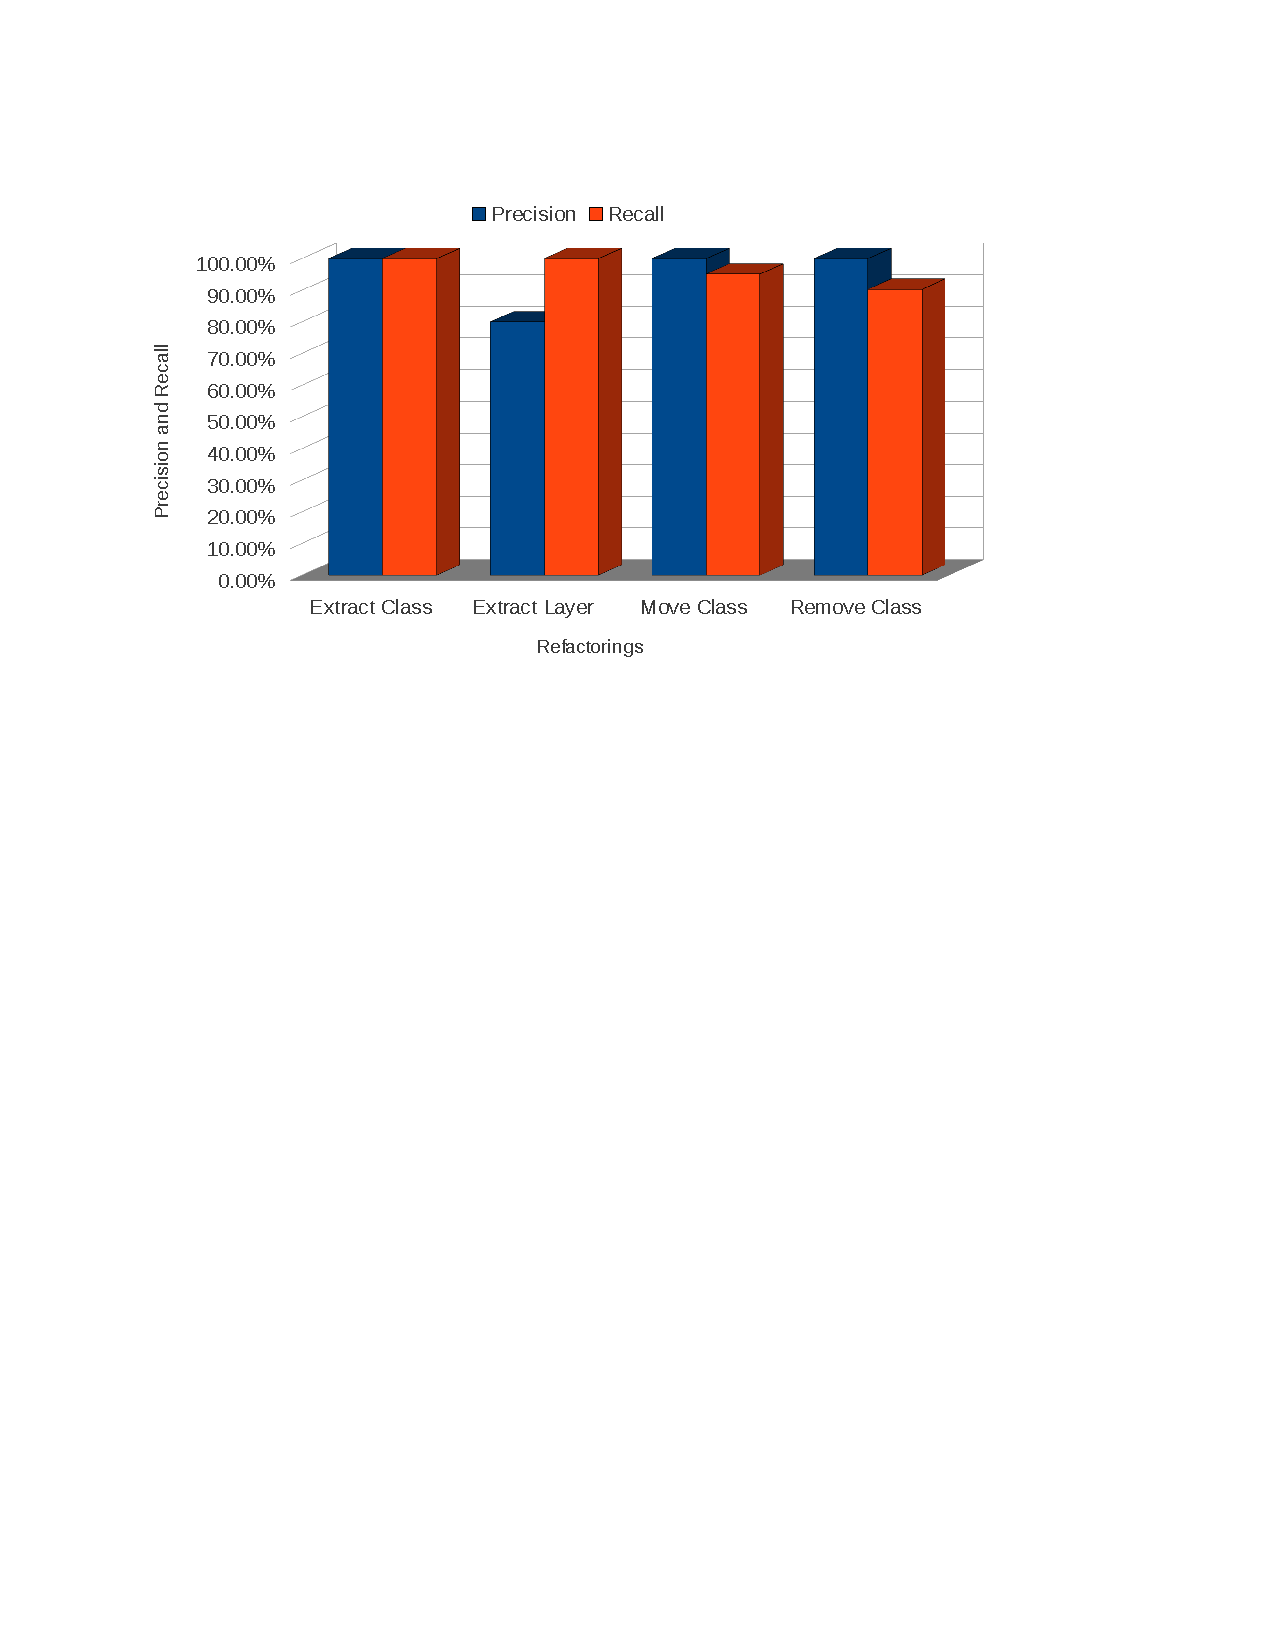
\includegraphics[scale=0.62]{figuras/barCharPrecisionAndRecall}
	\caption{Bar-plot for precision and recall of each refactoring.}
	\label{fig:charPrecisionAndRecall}
\end{figure}

Observing  both Table~\ref{table:precision_recall} and Figure~\ref{fig:charPrecisionAndRecall}, it is possible to see that for the refactoring \textit{Extract Class}'s parameters we got 100\% of precision and recall; that is there are no false negatives or positives. However, notice we got 80\% of precision for the refactoring \textit{Extract Layer}'s parameters. This happened because our mining algorithm has recognized more similar meta-classes in \textit{Extract Layer} than in \textit{Extract Class} increasing the number of false positives, as most of these meta-classes had not relation with the parameters.
%
Obviously, our MDI Algorithm failed in some cases because although some meta-classes are similar, the semantic is completely different. For example, we could have two similar instance of an specific meta-class, therefore the algorithm would identify just one. %However, it also clustered correctly the variable oafee that is a persistence field. 
As can be seen in Table~\ref{table:precision_recall} it is clear that our MDI Algorithm helps to find meta-classes which are related with a particular refactoring but it is not foolproof. Nevertheless, empirically we can say that the algorithm add value to the whole solution.

As can be seen in our analyses, good recall and precision values were obtained using our MDI Algorithm. Therefore, this can enable other groups to proceed researching on data mining techniques in KDM models. Thereby, the \textbf{RQ$_{experiment}$} can be answered as true, that is, the MDI Algorithm can be able to identify correctly the affected KDM elements. Clearly, we cannot guarantee the same level of recall and precision but maybe it is possible to keep improving these metrics by using other data mining techniques.

\subsection{Threats to Validity}

The lack of representativeness of the subject programs may pose a threat to external validity. We argue that this is a problem that all software engineering research, since we have theory to tell us how to form a representative sample of software. %Apart from not be- ing of industrial significance, another potential threat to the external validity is that the investigated pro- grams do not differ considerably in size and complex- ity. To partially ameliorate that potential threat, the subjects were chosen to cover a broad class of applica- tions. 
Also, this experiment is intended to give some evidence of the efficiency and applicability of our implementation solely in academic settings. A threat to construct validity stems from possible faults in the implementations of the techniques. With regard to our mining techniques, we mitigated this threat by running a carefully designed test set against a complex system.

%!TEX root = /Users/rafaeldurelli/Dropbox/Artigos Elaborados/KDM propagation_2015/sbes_2015_kdm_propagation/sbes2015_kdm_propagation.tex

The focus of our paper is the demonstration of propagation that must be performed in different static representations (views) of a given system. This means that we are not concerned with dynamic parts.
As stated earlier, previous research has demonstrated concerns about the propagation of changes when modifications are made in models. However, the largest of them are concentrated in the propagation of changes between different metamodels. As KDM is a integrated model that can be seen as a set of metamodels, where all of them are somehow connected by means of associations. This is because a certain model element is used in several places in general is referenced by its \textit{id} without having to be duplicated in multiple locations. However, as stated before, to the best of our knowledge, up to this moment, there is no research concentrated on investigating change propagation in KDM. We claim that by using our approach the modernization engineers can concentrate just on the development of the refactorings, without worrying about the change propagation, which is a time-consuming and error-prone task.

%Some partial change propagations are already developed by MoDisco\footnote{https://eclipse.org/MoDisco/} plugin. For example, when a particular model element is removed, its \textit{id} is removed from all the other places that it is used. This is considered a partial propagation, because it can, in most cases, inserting inconsistencies in the model. However, when dealing with specific refactorings it is important to keep all KDM levels synchronized 

During the elaboration of this research we realized that some propagations can also be considered as refactoring and vice versa. What characterize them is how they are used in a specific moment and not the implementation by itself. This is like having a set of refactoring that anyone can trigger anyone. When this is the case, the modernization engineer can directly apply both, unlikely propagations which clearly cannot be directly applied from the user, as it is shown in~\cite{ICSOFT2014_Winetzhammer}. This is generally the case for moving refactorings, as the moving of an element from a container to another is independent of both the container and their abstraction level. For example, suppose the existence of a class C1 belonging to a package P1. Consider also that C1 is the implementation of a business rule B1 which is inside a scenario S1 and that the package P1 is the implementation of the Scenario S1. So, C1 = B1 and P1 = S1. If the \textit{Move Class} refactoring is applied to transfer the class C1 to package P2, a natural propagation is to transfer the business rule B1 to another scenario. However, if the modernization engineer is using a modeling environment which provides a business rule view, (s)he could also have available for him(her) a moving business rule refactoring. In this case, the natural propagation would be to transfer the corresponding classes from one package to another. Therefore, we can see that in some cases there is bidirectional flow, which can be started from any point. 
%
%
%
The most important thing about this discussion is that this categorization lead us to make good designs in terms of refactorings and propagations. That is, for refactorings that fall in this category, it is very important to implement them as separated and decoupled modules which can be called directly from the user. So, all of our refactorings were implemented like that. 


\section{Related Work}\label{sec:related_work}
		%!TEX root = /Users/rafaeldurelli/Dropbox/Artigos Elaborados/KDM propagation_2015/sbes_2015_kdm_propagation/sbes2015_kdm_propagation.tex


%In~\cite{4440135}, Enrico Biermann et al. propose to use the Eclipse Modeling Framework (EMF), a modeling and code generation framework for Eclipse applications based on structured data models. They introduce the EMF model refactoring by defining a transformation rules applied on EMF models. EMF transformation rules can be translated to corresponding graph transformation rules. If the resulting EMF model is consistent, the corresponding result graph is equivalent and can be used for validating EMF model refactoring. Authors offer a help for developer to decide which refactoring is most suitable for a given model and why, by analyzing the conflicts and dependencies of refactorings. This initiative is closed to the model driven architecture (MDA) paradigm~\cite{Kleppe:2003} since it starts from the EMF metamodel applying a transformation rules.

%In~\cite{Rui:2003} Rui, K. and Butler, apply refactoring on use case models, they propose a generic refactoring based on use case metamodel. This metamodel allows creating several categories of use case refactorings, they extend the code refactoring to define a set of use case refactorings primitive. This refactoring is very specific since it is focused only on use case model, the issue of generic refactoring is not addressed, and these works do not follow the MDA approach.

%Another work on model refactoring is proposed in~\cite{Zhang05genericand}, based on the Constraint-Specification Aspect Weaver (C-SAW), a model transformation engine which describes the binding and parameterization of strategies to specific entities in a model. Authors propose a model refactoring browser within the model transformation engine to enable the automation and customization of various refactoring methods for either generic models or domain-specific models. The transformation proposed in this work is not based on any metamodel, it is not an MDA approach.

%------------------------------------------


Westfechtel \textit{et al}.~\cite{ICSOFT2014_Winetzhammer} presented an approach for refactoring static models (UML class diagrams) and propagate the changes to behavioral models (UML Sequence diagrams), aiming to maintain the consistency between these models. Unlikely these authors, in this project our goal is to propagate the changes to other static views, all of them belonging to the same family of metamodels. Considering that our approach does take into consideration behavior aspects, only static ones, we believe that both approaches are complementary to each other.

Egyed~\cite{Egyed:2006:ICC:1134285.1134339} proposed an UML-based approach similar to our first step, which is the mining and identification of model elements to be changed. In order to find those model elements, the author employs "consistency rules" between models. These rules always must keep satisfied when the models as synchronised/aligned. So, whenever an element is refactored, a broken rule is an indication that a desynchronisation problem occurred, allowing the identification of model elements that must be updated to synchronise the model again. The author argue that his approach scales up to large, industrial UML models. The author employs a strategy different from ours for the identification of the points to be updated; while we rely on the comparison between the original and refactored models, he relies on the consistency rules. We believe that the problem with his approach is the insertion of another task to be performed (the specification of the consistency rules), in which new problems and errors can be inserted. Our approach is more time-consuming in terms of processing, but we believe that the recall and precision of the identification is higher.

Therefore, to be best of our knowledge our work is the first one in presenting an approach for propagating changes in KDM models in a consistent and transparent way. The most fundamental differences of other related works are: i) we consider only static models, i.e, other views of the system; ii) we work with a family of metamodels that share a consistent and homogeneously terminology (syntax) and iii) our solution is KDM-specific and iv) our approach is tool supported by means of an Eclipse Plug-in which can be coupled to any refactoring scripts written in any transformation language. 

%----------------------------------------------------------------

%We are aware of only a few approaches dealing with the propagation of changes from the structural model into the behavioral model. Rosner and Bauer~\cite{murduck}  propose an approach to update model transformations in response to metamodel changes. The approach requires an ontology mapping between metamodel versions and is applied to evolve QVT-R~\cite{QVT} transformations. Similarly, Westfechtel \textit{et al}.~\cite{ICSOFT2014_Winetzhammer} presented an approach for refactoring static models (UML class diagrams, for example) and propagate the static changes to behavioral models (UML Sequence diagrams, for example), aiming to maintain the consistency between these models. Unlikely these authors, in this project our goal is to propagate the changes to other static views. It is not the purpose of our paper ensure that the refactorings maintain the observable behavioral of the system. Therefore, we believe that our approach are complementary to the proposal of the mentioned authors. 

%Recently, Egyed~\cite{Egyed:2006:ICC:1134285.1134339} proposed a very efficient approach to check for propagation (i.e. violations of consistency rules) in UML models. His approach scales up to large, industrial UML models by tracking which entities are used to check each consistency rule, and then using this information to determine which rules might be affected by a change, and only re-evaluate these rules. This work is complementary to our work: it provides a rapid means of checking consistency (which supports the first step of our approach), but does not tackle the issue of how to restore consistency.

%Research on model refactoring primarily focuses on the structural model (UML Class Diagrams). For example, in~\cite{4440135} refactoring of Ecore models is specified with graph transformation rules in the AGG environment. Differently our approach focus of model refactoring to KDM models.

%Altogether, the work presented in this paper is unique since it does not only support refactoring in KDM, but also keep all KDM levels synchronized by means of a decoupled set of ATL rules. Refactoring and propagation of changes in KDM levels are supported in an integrated/transparent way, i.e., after a refactoring changes are propagated to others KDM levels such that consistency and synchronization are preserved.

%In the line of language independent refactoring and metamodelling, Sander et al.~\cite{Tichelaar00}, study the similarities between refactorings for Smalltalk and Java, and build the FAMIX model. It provides a language-independent representation of object- oriented source code. It is an entity-relationship model that models object-oriented source code at the program entity level, with a tool to assist refactoring named MOOSE. FAMIX does not take account neither complex features in strongly typed languages, nor aspects of advanced inheritance and genericity. This approach is not really independent from language since the refactoring transformation is achieved directly on the original code. This alternative forces to implement transformers of specific code for each language. These code transformers use an approach based on text using regular expressions.




\section{Conclusions and Future Work}\label{sec:conclusion}
		%!TEX root = /Users/rafaeldurelli/Dropbox/Artigos Elaborados/KDM propagation_2015/sbes_2015_kdm_propagation/sbes2015_kdm_propagation.tex


The focus of our paper is the demonstration of propagation that must be performed in different static representations (views) of a given system. This means that we are not concerned with dynamic parts. As stated earlier, previous research has demonstrated concerns about the propagation of changes when modifications are made in models. However, the largest of them are concentrated in the propagation of changes between different meta-models. Otherwise we are interested in propagation of changes in different KDM abstraction views to keep them synchronized after a specific refactoring.   
%
%
We claim that by using our approach the modernization engineers can concentrate just on the development of the refactorings, without worrying about the change propagation, which is a time-consuming and error-prone task. 

As KDM is a integrated model that can be seen as a family of meta-models, where all of them are somehow connected by means of associations a certain model element is used in several places in general is referenced by its \textit{id} without having to be duplicated in multiple locations. This means that by applying the refactoring \textit{Rename X}, where X is any KDM elements the propagation would be performed automatically. During the elaboration of this research we also realized that some propagations can also be considered as refactoring and vice versa. What characterize them is how they are used in a specific moment and not the implementation by itself. This is like having a set of refactoring that anyone can trigger anyone. When this is the case, the modernization engineer can directly apply both, unlike propagations which clearly cannot be directly applied from the user, as it is shown in~\cite{ICSOFT2014_Winetzhammer}. This is generally the case for moving refactorings, as the moving of an element from a container to another is independent of both the container and their abstraction level. For example, suppose the existence of a class C1 belonging to a package P1. Consider also that C1 is the implementation of a business rule B1 which is inside a scenario S1 and that the package P1 is the implementation of the Scenario S1. So, C1 = B1 and P1 = S1. If the \textit{Move Class} refactoring is applied to transfer the class C1 to package P2, a natural propagation is to transfer the business rule B1 to another scenario. However, if the modernization engineer is using a modeling environment which provides a business rule view, (s)he could also have available for him(her) a moving business rule refactoring. In this case, the natural propagation would be to transfer the corresponding classes from one package to another. Therefore, we can see that in some cases there is bidirectional flow, which can be started from any point.  

  A certain particularity of our approach is that the required input is two KDM instances; the original and the refactored. As the refactoring activity is not part of our approach, there is no guarantee that other modernization engineers will implement refactorings that result in two models. Other possibilities would be having other kinds of inputs, such as an annotated KDM, or an extended KDM, or an stereotyped KDM. However, this will require modifications in our first step. 
 
Although our main focus along the paper had been on the lower-level refactorings and botton-up propagations, in our case study we decided to start an investigation on top-down propagations employing the \textit{Extract Layer} refactoring. The results seems to indicate that our propagation module is able to propagate correctly even in this case, as shown in Table~\ref{tab:prop}. However, we intend to deepen much more in this line of thought in a future work. Similarly, during the experiment carried out our MDI Algorithm seem to identify correctly the affected KDM elements, it reached a good level of precision and recall. However, we aim to pursue another mining techniques in future work.


%Although our main focus throughout the paper was lower-level refactorings and botton-up propagations, in our case study we investigated top-down propagations employing the \textit{Extract Layer} refactoring. The results seems to indicate that our propagation module is able to propagate correctly even in this case, as shown in Table~\ref{tab:prop}. However, we aim to pursue this approach in future work.

%The main contributions are: i) a DI Algorithm to identify all KDM model elements that need to be updated when a specific refactoring is performed, ii) a propagation technique approach, and (iii) a support and preliminary infrastructure for allowing the creation of refactorings for KDM without worrying about he propagation of changes.

Summing up, the idea behind KDM is that the community starts to create parsers and tools that work exclusively over KDM instances; thus, every tool/algorithm that takes KDM as input can be considered platform and language-independent. For instance, a refactoring catalogue for KDM~\cite{IRIDurelliCatalogo}, a crosscutting concerns mining for KDM models~\cite{dani_san}, architectural conformance checking for KDM models, could be applied to any system implemented in any language. In the same line of thought , an important point is about the reusability of the algorithms and transformations developed in this work. All of them are strictly focused on the KDM syntax, what makes them language and platform independent. So, we could use our propagation approach during the refactoring of systems implemented in C++, C\#, Cobol, etc in order to keep all their views synchronized.

\section*{Acknowledgments}
	%!TEX root = /Users/rafaeldurelli/Dropbox/Artigos Elaborados/KDM propagation_2015/sbes_2015_kdm_propagation/sbes2015_kdm_propagation.tex
Rafael Serapilha Durelli would like to thank the financial support provided by FAPESP, process number 2012/05168-4. Fernando Chagas and Bruno Santos would also like to thank CNPQ.


